% =====================================================================
%  Investigating the Sim-to-Real Gap in RGB-D Based Tabletop Pose
%  Estimation and Manipulation  --  M. M. Szokedencsi (s5173191), RUG BSc AI
%
%  SELF-CONTAINED build: compiles in Overleaf out-of-the-box (no custom .sty).
%  Citation style: APA via apacite (the official RUG BSc-AI template default).
%  Each chapter lives in sections/ ; appendices in appendix/ (\input below).
%
%  BUILD: pdfLaTeX -> BibTeX -> pdfLaTeX x2   (Overleaf "Recompile" handles it)
% =====================================================================
\documentclass[10pt,a4paper,twocolumn]{article}

\usepackage[utf8]{inputenc}
\usepackage[T1]{fontenc}
\usepackage[a4paper,margin=2cm]{geometry}
\usepackage{graphicx}
\usepackage{booktabs}
\usepackage{subcaption}
\usepackage{dblfloatfix}   % fix double-column figure* ordering so it doesn't block single figures
\usepackage{amsmath,amssymb}
\usepackage{siunitx}
\usepackage{apacite}            % APA author-year citations
\usepackage[hidelinks]{hyperref}

% --- more generous float placement so figures/tables stay near their text ---
\setcounter{topnumber}{3}
\setcounter{bottomnumber}{2}
\setcounter{totalnumber}{5}
\renewcommand{\topfraction}{0.92}
\renewcommand{\bottomfraction}{0.85}
\renewcommand{\textfraction}{0.06}
\renewcommand{\floatpagefraction}{0.7}

\graphicspath{{figures/}}

\begin{document}

% ========================= TITLE PAGE =========================
\begin{titlepage}
\centering
\vspace*{2.3cm}
{\Huge\bfseries Investigating the Sim-to-Real Gap in RGB-D Based Tabletop Pose Estimation and Manipulation\par}
\vspace{1.3cm}
{\Large Bachelor's Thesis\par}
\vspace{0.25cm}
{\large in Artificial Intelligence\par}
\vspace{2.6cm}
{\large\itshape Author\par}
\vspace{0.2cm}
{\Large Marcell Mor Szokedencsi\par}
\vspace{0.15cm}
{\large s5173191 \quad m.m.szokedencsi@student.rug.nl\par}
\vspace{1.6cm}
{\large\itshape Supervisor\par}
\vspace{0.2cm}
{\Large Dr.\ H.\ Kasaei\par}
\vfill
{\large University of Groningen\par}
\vspace{0.15cm}
{\large Bernoulli Institute \textemdash\ Faculty of Science and Engineering\par}
\vspace{0.9cm}
{\large \today\par}
\end{titlepage}

% =========== full-width abstract, above the two-column body ===========
\twocolumn[%
\begin{center}
{\Large\bfseries Abstract}
\end{center}
\begin{center}
\begin{minipage}{0.93\textwidth}
\small\noindent
Vision-based manipulation systems are usually developed in simulation and then
transferred to hardware, where they often degrade. A frequently cited cause of this
sim-to-real gap is sensor mismatch, particularly depth noise that simulated RGB-D
streams fail to reproduce. This thesis presents a controlled study of how realistic
Time-of-Flight (ToF) depth noise affects a fixed top-down tabletop pipeline for pose
estimation and pick-and-place, using a Luxonis OAK-D SR PoE camera and a low-cost
xArm~1S arm in a Gazebo Classic and ROS~2 stack. We characterise the real sensor,
inject a four-term ToF noise model into the simulated depth, and evaluate pose accuracy
and grasping in clean simulation, noisy simulation, and on the real robot. The headline
result is negative: for a depth-segmented median-centroid estimator, injecting noise at
the measured level has no measurable effect on pose RMSE (below \SI{0.1}{\milli\metre}
versus clean) and none on grasp success, because the per-axis median discards the edge
flying-pixels that carry the real noise. Accuracy degrades only when the axial term is
scaled roughly tenfold, a regime characteristic of harsh, hot, or outdoor ToF operation
rather than the controlled indoor setting studied here; this verifies that the null
reflects the estimator, not a broken pipeline. The real system confirms the simulation:
a planar pose gap of $-1.4$ to $+3.6$\,mm across four objects and a 57\% closed-loop
grasp success rate, with per-object outcomes set by grip mechanics rather than depth
noise. We conclude that, for an outlier-robust estimator, the sim-to-real gap here is
dominated by calibration and lighting rather than depth-noise-model fidelity.
\end{minipage}
\end{center}
\vspace{1.2em}
]

% --- chapters (one file each) ---
\section{Introduction}
RGB-D perception is a standard building block for object localisation and robotic
manipulation. Because real robot time is slow, fragile, and expensive, a large share of
this work is developed in simulation and only later moved onto hardware. The recurring
difficulty is that pipelines which behave well in simulation often lose accuracy or fail
outright once they meet a real sensor and a real arm. This discrepancy is known as the
reality gap or sim-to-real gap, and it was already identified in evolutionary robotics
three decades ago, where the role of noise in bridging the gap was made explicit
\cite{jakobi1995noise}. A common modern response is domain randomisation, which
deliberately varies simulator parameters so that the real world looks like one more
sample of the training distribution \cite{tobin2017domain}. Randomisation is effective
but blunt: it rarely tells us which mismatch actually mattered in a given setup.

This thesis isolates a single, measurable source of mismatch in a deliberately
constrained setting. We use a fixed top-down camera over a tabletop, so the dominant
uncertainty is depth sensing rather than viewpoint or hand-eye drift. The camera is a
Time-of-Flight (ToF) device, whose depth error depends on range, surface properties, and
scene geometry. The question we ask is narrow and quantitative: if we measure the real
ToF noise and inject a faithful model of it into simulation, does the simulated
pose-estimation and grasping behaviour move closer to the real system?

The answer we report is, for this pipeline, no, and we argue that this negative result is
the most useful outcome of the project. The perception component is a classical,
outlier-robust estimator, and it turns out to absorb realistic ToF noise almost
completely. Rather than treat that as a failure, we quantify exactly how much noise the
estimator tolerates before it breaks, show that the breaking point sits an order of
magnitude above reality, and confirm on the real robot that the simulated conclusion
holds end to end. The practical message is that, for an estimator of this kind, effort
spent on high-fidelity depth-noise models is misdirected; the residual gap lives
elsewhere, in calibration and lighting.

\subsection{Research Questions}
The work is organised around one main research question and three sub-questions.

\noindent\textbf{Main RQ.} How does modelling realistic Time-of-Flight (ToF) sensor
noise affect the sim-to-real gap in RGB-D tabletop pose estimation and manipulation?
\begin{itemize}
  \item \textbf{SQ1 (noise statistics).} What is the real ToF sensor's noise behaviour,
  and how well do literature models (Nguyen 2012, Kinect-class) describe it? Addressed in
  Phase~2.
  \item \textbf{SQ2 (pose accuracy).} Does injecting measured noise into simulation
  change pose-estimation accuracy relative to clean simulation? Addressed in Phase~3.
  \item \textbf{SQ3 (manipulation propagation).} To what extent do pose estimation errors
  propagate to manipulation performance (pick success rate and placement accuracy)?
  Addressed in Phases~4A (simulation), 4B (real perception), and 4C (real manipulation).
\end{itemize}

\subsection{Hypothesis}
The proposal stated the directional hypothesis that injecting measured ToF noise into
simulation will reduce the sim-to-real gap. As the results show, this hypothesis is not
confirmed at realistic noise levels. We treat the refutation as a finding in its own
right and design the later phases to test whether the same null carries from pose
estimation through to manipulation.

\subsection{Contributions}
\begin{enumerate}
  \item A measured ToF noise characterisation of the OAK-D SR PoE in a fixed top-down
  tabletop setup, including the finding that bulk (body) depth is sub-millimetre and
  essentially flat with range, while edge flying-pixels dominate the pose-relevant error.
  \item A practical depth-noise injection module that implements four literature ToF
  terms (axial Gaussian, lateral jitter, edge mixed-pixels, and dropout) and exposes an
  axial-scale control for ablation.
  \item The central, controlled result: at the measured sensor noise level, the injected
  noise has no measurable effect on pose RMSE or on grasp success for a depth-segmented
  median-centroid estimator. Degradation appears only at roughly ten times the measured
  axial noise for pose and roughly twenty times for manipulation. Because the injector
  demonstrably breaks perception when scaled far enough, the null is sound rather than an
  artefact.
  \item End-to-end validation on the real system: a real-versus-sim planar pose gap
  between $-1.4$ and $+3.6$\,mm across four objects, and a 60-trial real closed-loop
  pick-and-place (34/60 lifts) showing that, once visual feedback corrects the aiming
  error, real grasp success is governed by object grip mechanics rather than by depth
  noise or the simulated pose-error propagation.
  \item A reproducible Gazebo Classic and ROS~2 tabletop manipulation setup for the
  xArm~1S with an overhead RGB-D sensor.
\end{enumerate}
It is important to be precise about scope. The pick-and-place component is the proposal's
authorised predefined grasp strategy for known object types; it is a baseline used to
test whether the pose-level null propagates to grasping, and it is not presented as a
novel system. The engineering of the real closed-loop executor (Phase~4C) is reported as
methods and appendix material, not as a results contribution.

\subsection{Thesis Outline}
Section~\ref{sec:related} reviews related work. Section~\ref{sec:methods} describes the
simulation, the noise characterisation protocol, the injection model, the perception and
grasp pipelines, and the real-world calibration and control. Section~\ref{sec:setup}
specifies the hardware, objects, conditions, trial counts, and metrics.
Section~\ref{sec:results} reports the results. Section~\ref{sec:discussion} interprets the
negative result and its limitations, and Section~\ref{sec:conclusion} concludes and
outlines future work.

% =====================================================================

\section{Related Work}\label{sec:related}
\subsection{The sim-to-real gap and domain randomisation}
The gap between simulated and real robot behaviour is a long-standing concern. Early work
in evolutionary robotics framed it as the reality gap and argued that controllers
transfer only when the simulator captures the right sources of variation, with noise
playing a central role in preventing overfitting to simulator artefacts
\cite{jakobi1995noise}. Domain randomisation generalises this idea by sampling simulator
parameters such as textures, lighting, and dynamics, so that the real world appears as
one more draw from a broad training distribution \cite{tobin2017domain}. Such methods are
powerful for learned systems but are typically applied as a blanket strategy; they do not
attribute the residual gap to a specific physical cause. This thesis takes the
complementary, analytic route of isolating one cause, ToF depth noise, and measuring its
effect directly.

\subsection{ToF and depth-sensor noise modelling}
Depth sensors have well-studied, sensor-specific error characteristics. Structured-light
and ToF cameras differ markedly, and ToF noise in particular is shaped by integration
time, multipath, and surface reflectance \cite{sarbolandi2015kinect,foix2011lockin}. For
consumer depth cameras, a widely used axial-and-lateral model expresses the depth
standard deviation as a function of range and viewing angle \cite{nguyen2012modeling},
while empirical characterisations of Kinect-class sensors report range-dependent
precision and systematic bias \cite{khoshelham2012accuracy}. A recurring finding is that
a large fraction of usable error concentrates at depth discontinuities as flying or mixed
pixels \cite{foix2011lockin,sarbolandi2015kinect}. We adopt these models as the expected
behaviour that our own measurements test, and we report where they do and do not hold for
the OAK-D SR PoE.

\subsection{Tabletop perception and pose estimation}
Classical tabletop perception pipelines segment objects from a dominant support plane,
often by fitting the plane with RANSAC and clustering the remaining points
\cite{rusu2008towards}. When the support surface is known and fronto-parallel, as in our
fixed overhead setup, the plane fit can be replaced by a simpler depth threshold; we make
this substitution deliberately and cite the RANSAC-based pipeline only as a point of
contrast. For evaluating pose, the BOP benchmark consolidated metrics and datasets for 6D
object pose \cite{hodan2018bop}; we use only its notion of aligning the visible top
surface, because our estimator produces a translation-only (3-DoF) pose rather than a
full 6D pose with orientation.

\subsection{Fiducial markers for ground truth}
Establishing a real-world reference frame requires reliable fiducials. Square markers such
as ArUco provide robust, occlusion-tolerant detection \cite{garridojurado2014aruco}, and
fast detectors improve corner localisation and detection speed
\cite{romeroramirez2018charuco}. We use a printed ChArUco board (ArUco markers combined
with a chessboard) to recover the camera-to-table transform by direct \texttt{solvePnP},
and individual markers to obtain per-object ground-truth positions.

\subsection{Grasping}
Data-driven grasp synthesis spans analytic and learned approaches and is surveyed
comprehensively in \citeA{bohg2014grasp}; learned multi-view grasping in clutter is an
active line within the host lab \cite{kasaei2021mvgrasp}. Our work does not contribute a
grasping method. Consistent with the proposal, we use a fixed, predefined grasp for known
objects so that any grasp error is attributable to perception rather than to grasp
planning, and we use this baseline purely to test whether pose-level errors propagate to
pick success.

% =====================================================================

\section{System and Methods}\label{sec:methods}

All three depth sources---clean simulation, noise-injected simulation, and the real
OAK-D---feed a single shared perception$\rightarrow$IK$\rightarrow$grasp pipeline
(Figure~\ref{fig:pipeline}), so that depth noise is the only variable distinguishing the
conditions. The following subsections describe each stage in turn.

\begin{figure*}[t]
\centering
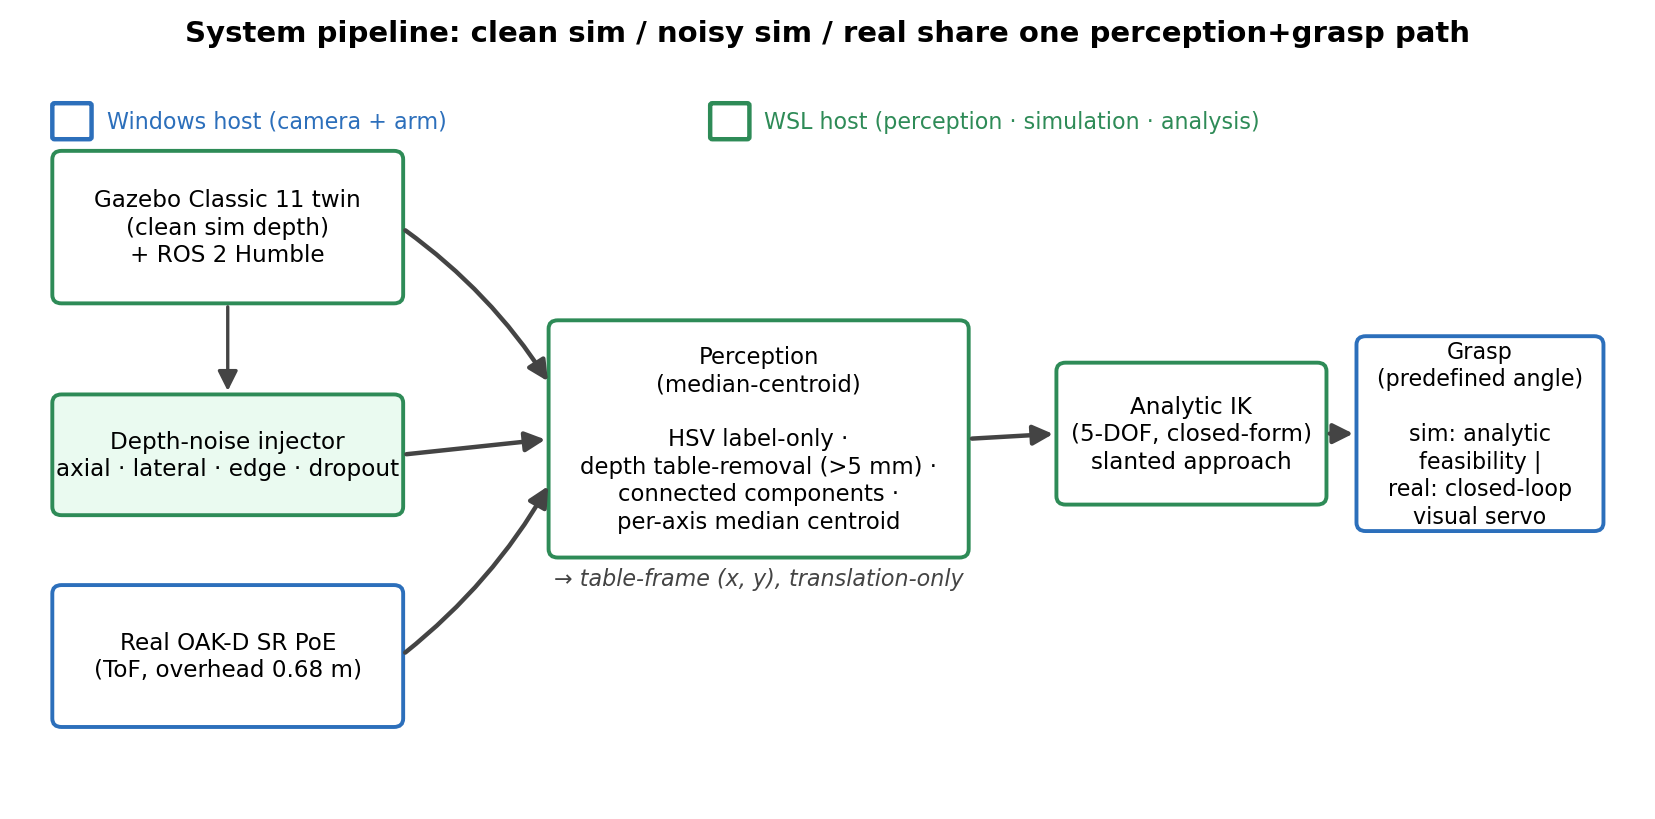
\includegraphics[width=0.92\textwidth]{system_pipeline.png}
\caption{System pipeline. Clean simulation, noise-injected simulation, and the real
OAK-D feed one shared perception$\rightarrow$IK$\rightarrow$grasp path, isolating depth
noise as the only variable. Box colour indicates the host: the camera and arm run on
Windows; perception, simulation, and analysis run under WSL.}
\label{fig:pipeline}
\end{figure*}

\subsection{Simulation and robot model}
The simulation uses Gazebo Classic~11 with ROS~2 Humble (Figure~\ref{fig:simscene}).
Control is provided through
\texttt{ros2\_control}, with a joint-trajectory controller for the arm and an effort/PID
controller for the gripper, integrated through a vendored build of
\texttt{gazebo\_ros2\_control} \cite{gazebo_ros2_control}. The arm is anchored to the
world by a fixed joint at $z=0.76$\,m so that it does not fall or drift, which keeps every
measured grasp error attributable to perception rather than to base motion.

The robot is a Hiwonder xArm~1S, a low-cost hobby arm. Its URDF was sourced from a
community model (GrabCAD; see Appendix~\ref{app:assets}) and modelled as a 5-DOF kinematic
chain followed by a parallel-jaw gripper: a base yaw joint, a planar three-revolute (3R)
sub-chain whose three pitch axes are parallel, and a wrist roll. The gripper is fixed
relative to the wrist, with the tool point offset $+0.09$\,m beyond the last
joint.\footnote{The proposal refers to the arm as 6-DoF; the implemented analytic
kinematics are 5-DOF, consistent with the URDF used.}

The camera is a Luxonis OAK-D SR PoE ToF unit \cite{luxonis_oakd}, mounted overhead and
pointing straight down at $0.68$\,m above the table. The same mount height is carried into
simulation, which removes eye-in-hand drift and isolates the depth axis as the variable of
interest. The stream is RGB-D at $640\times480$ with an approximately $60^\circ$ field of
view, accessed through DepthAI \cite{depthai_docs}; factory intrinsics are used
throughout, with no separate calibration run.

\begin{figure}[htbp]
\centering
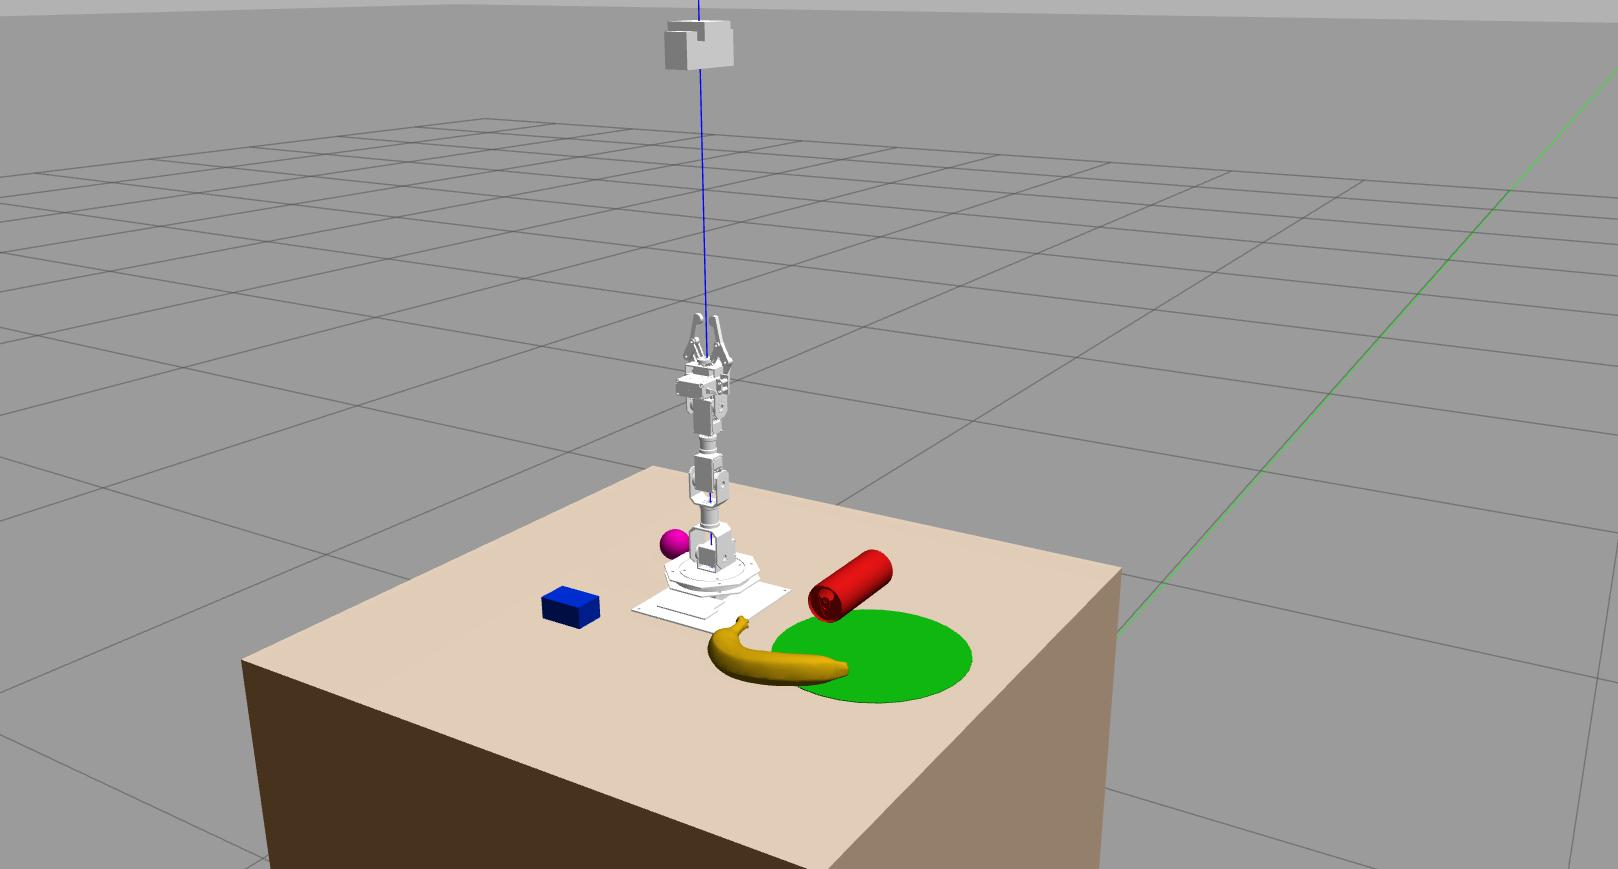
\includegraphics[width=\linewidth]{sim_scene.jpg}
\caption{The matched digital twin in Gazebo Classic: the simulated xArm~1S with its
parallel-jaw gripper over the tabletop, the four task objects (blue box, banana, red can,
and a sphere standing in for the golf ball), and the overhead OAK-D above. The same
geometry, mount height, and objects are used on the real system.}
\label{fig:simscene}
\end{figure}

\subsection{Analytic inverse kinematics}
Because the three pitch joints form a planar 3R arm, the arm position is solved in closed
form analytically in pure NumPy, following standard manipulator kinematics
\cite{craig2005robotics}, with an optional forward-kinematics cross-check. Avoiding a
numerical solver removes solver convergence as a confound, so any grasp error reflects
perception, not planning. A practical consequence of the table-mounted geometry is that a
purely vertical top-down grasp is infeasible at most reaches. A \texttt{feasible\_approach}
routine therefore searches for the steepest reachable slanted approach within the joint
limits; the achievable approach tilt degrades from near vertical close to the base to
roughly $70$--$80^\circ$ at far reach, which becomes relevant in the real manipulation
results.

\subsection{Real ToF noise characterisation}
The sensor was characterised with on-camera smoothing disabled so as to expose the raw
noise: the FPPN, optical, and wiggle corrections were left on, while the temporal and
median filters were turned off. Each capture aggregates 200 frames. Two protocols were
used. The planar protocol follows standard depth-camera characterisation practice
\cite{khoshelham2012accuracy}: a matte, fronto-parallel target is imaged at five distances
from $0.40$ to $0.80$\,m, and the per-pixel temporal standard deviation and bias are
estimated. The object protocol separates each object's body from a six-pixel edge ring,
motivated by the observation that ToF error concentrates at depth discontinuities as
flying or mixed pixels \cite{foix2011lockin,sarbolandi2015kinect}. Together these
protocols test how well the literature models \cite{nguyen2012modeling,khoshelham2012accuracy}
describe the OAK-D SR PoE in this setup.

\subsection{Depth-noise injection model}\label{sec:methods-inject}
The injector adds four literature noise terms, parameterised from the measured YAML, to
the clean simulated depth $z(u,v)$ before it reaches perception, which avoids modifying
Gazebo internals (Figure~\ref{fig:cleannoisy}). Writing the perturbed depth as $z'$, the
four terms are applied in sequence:
\begin{align}
\text{axial:}   &\quad z' = z + s\,\sigma_z(z)\,\eta, \label{eq:axial}\\
\text{lateral:} &\quad z'(u,v) = z\big(u+\Delta u,\,v+\Delta v\big), \label{eq:lateral}\\
\text{edge:}    &\quad z' = \alpha\,z_{\text{near}} + (1-\alpha)\,z_{\text{far}}, \label{eq:edge}\\
\text{dropout:} &\quad z' \to \varnothing. \label{eq:dropout}
\end{align}
In the axial term~\eqref{eq:axial}, $\eta\sim\mathcal{N}(0,1)$, $s$ is the axial-scale
multiplier, and the per-pixel standard deviation follows the Nguyen model
$\sigma_z(z)=a+b\,(z-z_0)^2$ \cite{nguyen2012modeling}. The lateral term~\eqref{eq:lateral}
resamples each output pixel from a neighbour offset by
$(\Delta u,\Delta v)\sim\mathcal{N}(0,\sigma_L^2)$, also from Nguyen, with the
incidence-angle term dropped because the overhead camera looks down the table normal
($\theta\approx0$) and $\sigma_L$ fixed to the literature value of $0.8$\,px. The edge
mixed-pixel term~\eqref{eq:edge} fires only at depth discontinuities, where
$\lvert\partial_u z\rvert+\lvert\partial_v z\rvert>\tau$, with probability $p_e$, replacing
the pixel by a convex mix ($\alpha\sim\mathcal{U}(0,1)$) of the nearest and farthest depth
in its $3\times3$ neighbourhood \cite{foix2011lockin,sarbolandi2015kinect}. The dropout
term~\eqref{eq:dropout} marks a pixel invalid with probability $p_d$, where $\varnothing$
denotes a dropped, no-return pixel \cite{sarbolandi2015kinect}.

The two noisy conditions differ only in their parameters. The measured model
\texttt{sim\_noisy\_oakd} sets $a=0.9$\,mm and $b=0$---a flat, range-independent axial
floor, consistent with the Phase-2 finding that the OAK-D's axial precision is
sub-millimetre and essentially flat with range---together with $\tau=2$\,cm, $p_e=0.70$ and
$p_d=0$, since no dropout was measured. The literature model \texttt{sim\_noisy\_nguyen}
instead uses Nguyen's Kinect coefficients $(a,b,z_0)=(0.0012,0.0019,0.4)$, $\tau=5$\,cm,
$p_e=0.30$ and $p_d=0.02$; both share $\sigma_L=0.8$\,px. To probe robustness, the axial
term is multiplied by an \texttt{axial\_scale} factor $s$ swept over $\{1,2,5,10,20\}$,
where $\times1$ is the measured level. The random number generator is seeded, with
independent streams for the continuous noise and the discrete masks, so that conditions are
directly comparable; the seeded ablation design is our own, in the spirit of controlled
randomisation studies \cite{tobin2017domain}. The third condition, \texttt{sim\_clean},
applies no injector.

\begin{figure}[htbp]
\centering
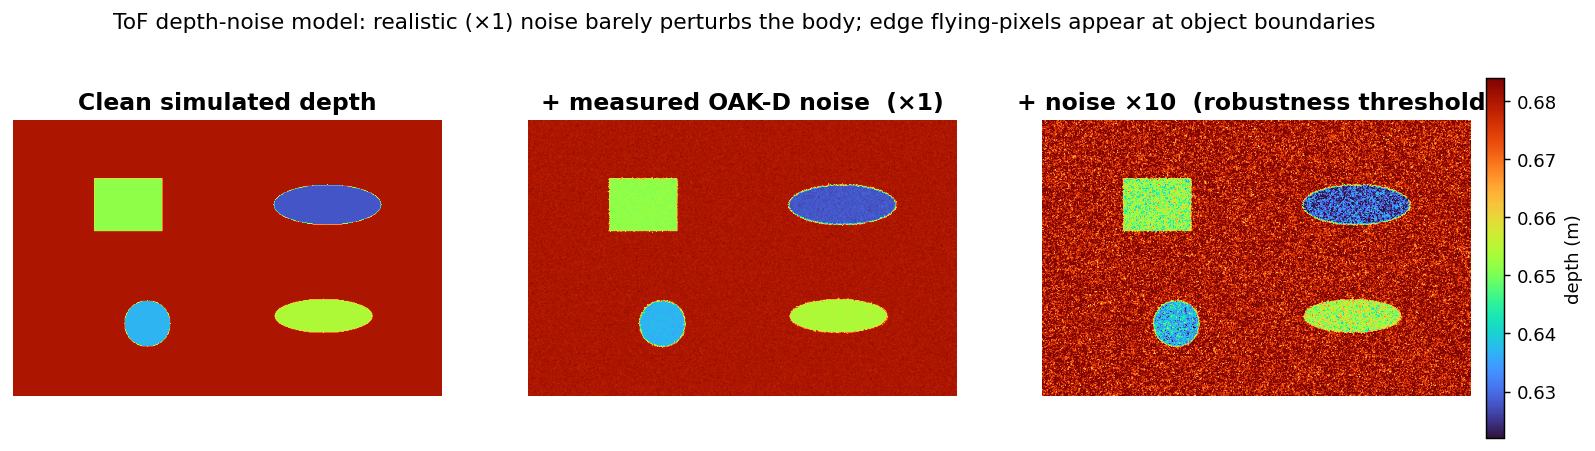
\includegraphics[width=\linewidth]{clean_vs_noisy_depth.png}
\caption{Simulated tabletop depth, clean versus the measured four-term ToF noise model
injected at $\times1$ and $\times10$. At the measured ($\times1$) level the object bodies
are barely perturbed and the added noise concentrates at edges; only at $\times10$ does
the field visibly degrade.}
\label{fig:cleannoisy}
\end{figure}

\subsection{Perception pipeline}\label{sec:methods-perc}
The perception module is classical and geometric by design. The RGB image is converted to
HSV and per-object colour masks are used only to label which blob is which; they never
contribute to geometry. The table is removed in depth: its plane depth is estimated as the
median of all valid depths, and any pixel at least $\delta=5$\,mm closer is marked as
object,
\begin{equation}
\begin{aligned}
z_{\text{table}} &= \operatorname{median}\{z(u,v)\},\\
\mathcal{O} &= \{(u,v): z(u,v)<z_{\text{table}}-\delta\}.
\end{aligned}
\label{eq:table}
\end{equation}
This step deliberately replaces RANSAC plane fitting \cite{rusu2008towards}, which is
unnecessary here because the support plane is known and fronto-parallel. Connected
components \cite{bradski2000opencv} then yield one blob per object. For each blob, the
valid pixels are back-projected with the pinhole intrinsics and reduced to a position by
the per-axis median of their coordinates,
\begin{equation}
\begin{aligned}
&X = (u-c_x)\,z/f_x,\quad Y = (v-c_y)\,z/f_y,\quad Z = z,\\
&\hat{\mathbf{c}} = \big(\operatorname{median}_i X_i,\ \operatorname{median}_i Y_i,\ \operatorname{median}_i Z_i\big),
\end{aligned}
\label{eq:median}
\end{equation}
giving a table-frame position (Figure~\ref{fig:perception}). The pose is translation-only
(3-DoF), with orientation set to identity.

The per-axis median is the crux of the entire study. It is an outlier-robust estimator
with a 50\% breakdown point \cite{huber1981robust}, and it is exactly what discards the
large edge flying-pixel population (between 53\% and 99\% of edge pixels, depending on
object) that constitutes the real noise. Finally, detections are matched to ground truth
by greedy nearest-neighbour assignment, a deliberate and documented simplification.

\begin{figure}[htbp]
\centering
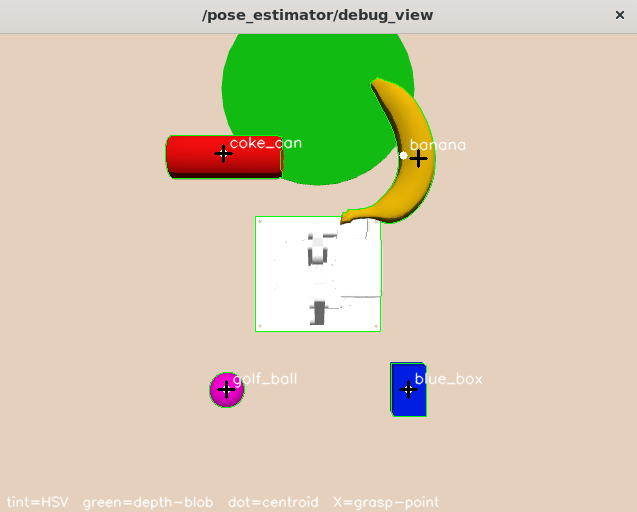
\includegraphics[width=\linewidth]{perception_debug.png}
\caption{Perception pipeline output (the \texttt{pose\_estimator} debug view): per-object
HSV colour labels (used only for identity, never for geometry), the depth blob (green), and
the per-object median centroid (dot) and predefined grasp point (X) for all four objects.
The position comes entirely from the depth blob; the colour tint never contributes to it.}
\label{fig:perception}
\end{figure}

\subsection{Grasp pipeline and feasibility metric}
Grasping uses a fixed, predefined per-object nominal grasp angle, identical in simulation
and on the real arm, which positions the predefined-grasp baseline discussed in the
grasping literature \cite{bohg2014grasp} rather than planning grasps online. Because
Gazebo Classic cannot reliably contact-grasp small or curved objects (finger collisions
pass through, and the object pose is bit-identical before and after closing the jaws), the
success metric is analytic rather than physical. A grasp is scored as feasible if and only
if the perceived object centre lies within the object's jaw capture tolerance of the true
centre, that is, if the open jaws would straddle the object. With per-object grasp width
$w$ and the measured gripper opening $W_{\text{jaw}}=55$\,mm, the jaw capture tolerance is
$\tau=(W_{\text{jaw}}-w)/2$, and feasibility is the planar test
\begin{equation}
\begin{aligned}
&\tau = (W_{\text{jaw}}-w)/2,\\
&e_{\text{cap}} = \lVert\hat{\mathbf{c}}_{xy}-\mathbf{c}^{*}_{xy}\rVert_2,\\
&\texttt{grasp\_feasible} = \mathbf{1}\!\left[\,e_{\text{cap}}\le\tau\,\right].
\end{aligned}
\label{eq:feasible}
\end{equation}
where $\hat{\mathbf{c}}_{xy}$ and $\mathbf{c}^{*}_{xy}$ are the perceived and true object
centres in the table plane. To avoid overclaiming, this metric is named
\texttt{grasp\_feasible} rather than pick success. For visualisation only,
a custom MIT plugin performs a contact-triggered fixed-joint attach following the
IFRA-Cranfield link-attacher pattern \cite{link_attacher}; it does not feed the measured
data.

\subsection{Real-world extrinsic calibration}\label{sec:methods-extrinsic}
For the real evaluation (Phase~4B), fiducials are detected on the OAK-D RGB camera rather
than on the ToF amplitude image, because the soft amplitude image yielded no usable
corners; the detections are then composed into the depth frame through the factory
RGB-to-ToF extrinsic. The camera-to-table transform is recovered from a printed
$7\times5$ ChArUco board (dictionary \texttt{DICT\_5X5\_100}, $100$\,mm squares) by direct
\texttt{solvePnP} \cite{garridojurado2014aruco,romeroramirez2018charuco}, with no hand-eye
calibration (Figure~\ref{fig:extrinsic}). The solution localised 20 of 24 corners at
$0.26$\,px reprojection error and placed the board at $0.683$\,m, in agreement to $1.4$\,mm
with the $0.684$\,m plane fitted to the depth image. Frame transforms are handled with the
ROS~2 transform library \cite{foote2013tf}.

\begin{figure}[htbp]
\centering
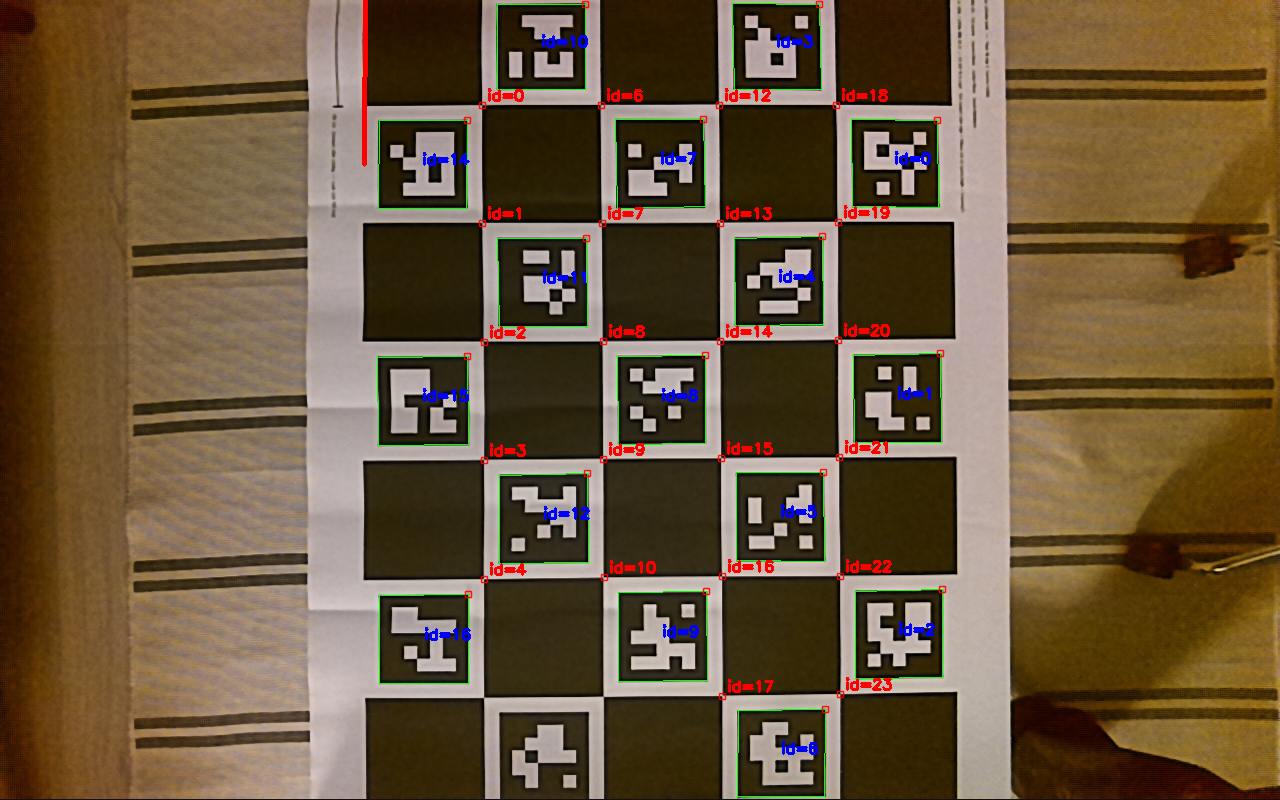
\includegraphics[width=\linewidth]{extrinsics_overlay.png}
\caption{The $7\times5$ ChArUco extrinsic board (\texttt{DICT\_5X5\_100}, $100$\,mm squares)
as imaged by the OAK-D's own RGB camera, with the OpenCV ArUco detection overlaid (green
marker boundaries, red ids). These marker and chessboard-corner correspondences feed the
direct \texttt{solvePnP} that recovers the camera-to-table extrinsic; the resulting board
height ($0.683$\,m) agrees with the depth-plane fit ($0.684$\,m) to $1.4$\,mm.}
\label{fig:extrinsic}
\end{figure}

\subsection{Real arm control and closed-loop visual servo}\label{sec:methods-servo}
The real arm is driven over USB-HID using a lightweight, ROS-free Python bridge. This
work, including the closed-loop executor below, is baseline and appendix material rather
than a results contribution; it exists so that the real grasp uses the same recipe as
simulation and the measured gap reflects execution rather than a perception confound. Two
real-to-model mismatches drive the design. First, the real gripper opens to $55$\,mm,
whereas the idealised URDF opened to $72$\,mm; the smaller real opening tightens the
tightest object's capture tolerance and is a disclosed source of sim-to-real difference.
Second, and more importantly, the real arm over-reaches the URDF kinematic model by
roughly 28\%,% TODO: confirm against the bench value -- the 0.777 scale implies 1/0.777 = 1.287, i.e. ~28.7% over-reach
 because the model link lengths do not match the physical arm. A global
similarity-scale table-to-arm transform of approximately $0.777$ (the reciprocal of the
over-reach factor, $1/1.287$) reduces this but leaves a
position-dependent residual of about $14$\,mm RMS over the workspace, which exceeds the
tightest object's tolerance and confines reliable open-loop grasping to a small patch of
the table.

The residual is an unidentifiable, position-dependent kinematic-model error, so no fixed
offset or low-parameter recalibration can remove it across the workspace. The adopted
solution closes the loop visually in a way that is independent of the broken kinematics
(Figure~\ref{fig:servo}). A single ArUco marker (dictionary \texttt{DICT\_4X4\_50}, id~4;
the object markers use ids 0--3) is taped flat on the gripper so the overhead camera sees
it. Before descending, the controller iterates in the table frame,
\begin{equation}
\mathbf{e} = \mathbf{p}_{\text{obj}} - \big(\mathbf{p}_{\text{marker}} + \mathbf{t}_{\text{tip}}\big),
\qquad \mathbf{target}\mathrel{+}= K\,\mathbf{e},
\end{equation}
with gain $K\approx0.6$, until $\lVert\mathbf{e}\rVert < 3$\,mm, after which it descends
and closes. Because the error is a difference of two points measured through the same
camera in the same frame, the incorrect forward kinematics and the global scale act as
common-mode bias and cancel; they only need to be good enough for the loop to converge.
Grasp accuracy then becomes camera-bound (on the order of $1$ to $4$\,mm) across the
workspace. A dense, camera-measured correction field, in the spirit of low-cost
reproducible-arm calibration work \cite{yang2019replab}, was prepared as a citable
open-loop fallback but was not needed, since the closed loop alone produced the result.

\begin{figure*}[t]
\centering
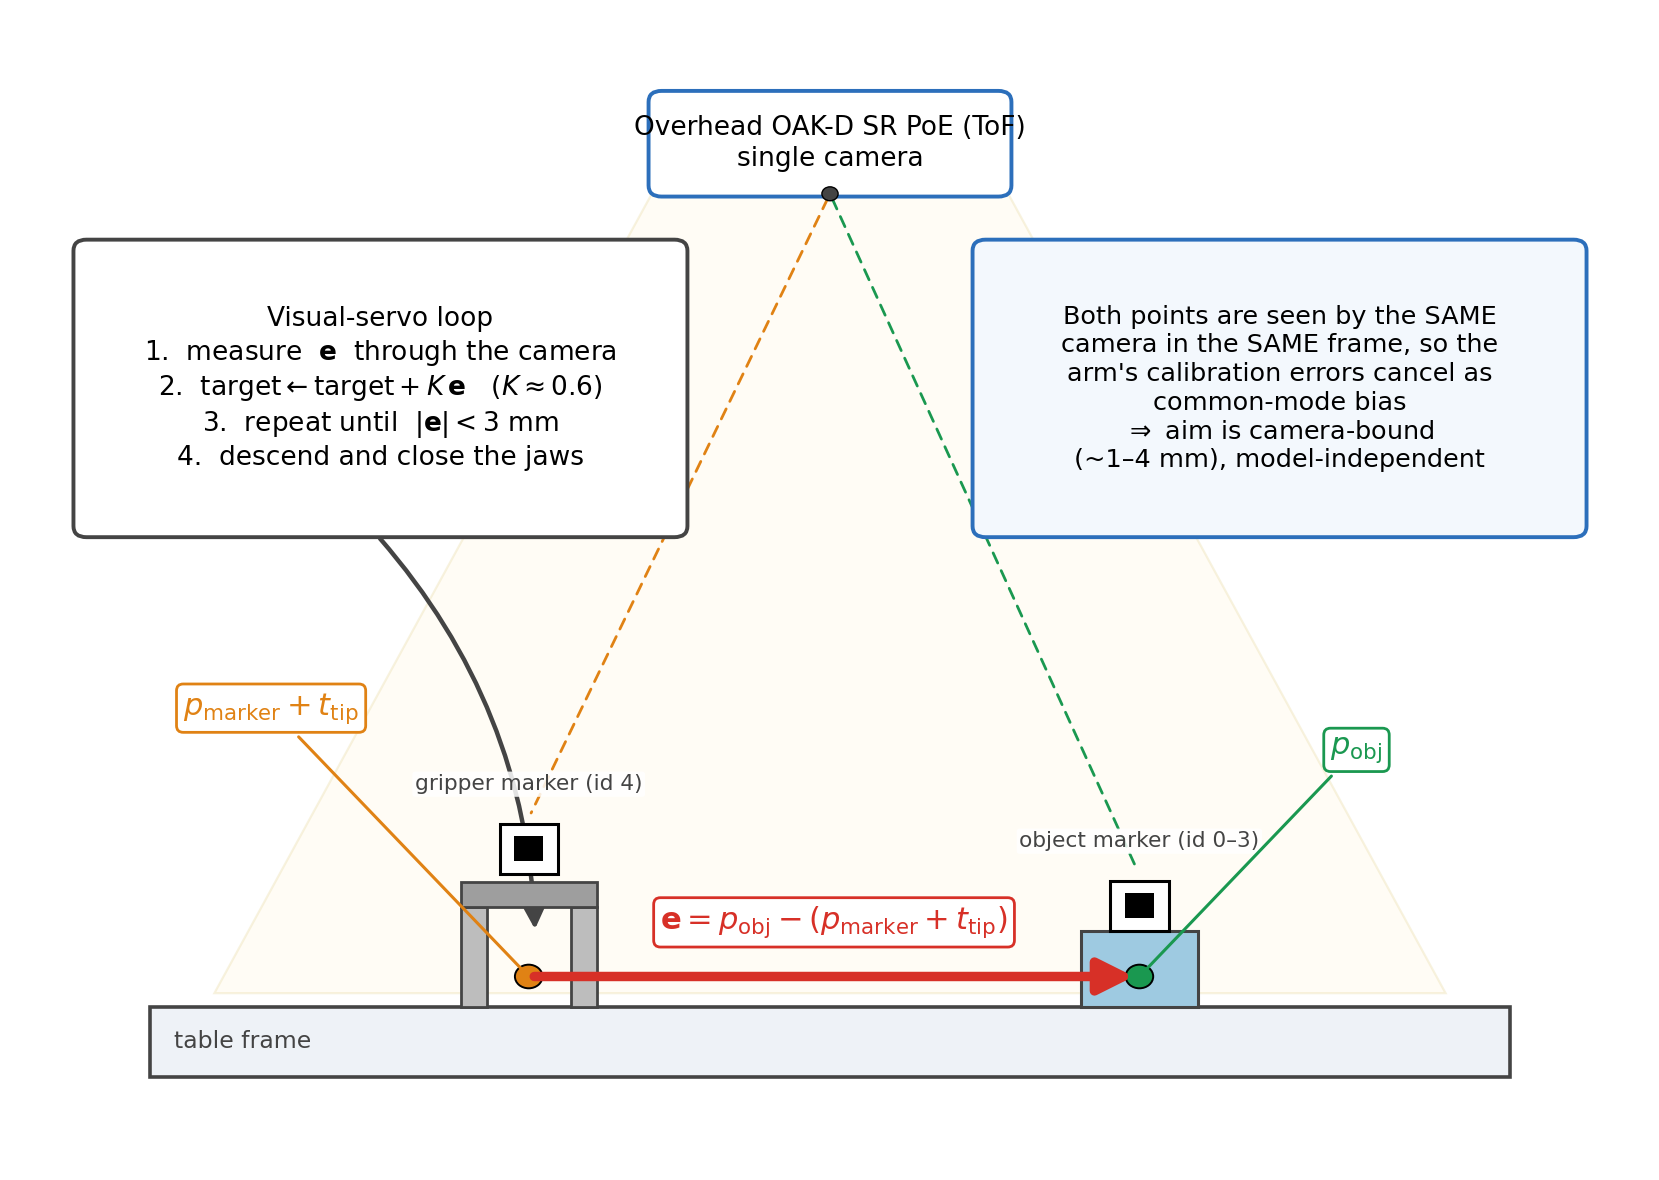
\includegraphics[width=0.86\textwidth]{servo_schematic.png}
\caption{Closed-loop visual-servo alignment (Phase~4C, baseline/Methods). The single
overhead camera measures the object point $\mathbf{p}_{\text{obj}}$ and the gripper-marker
point $\mathbf{p}_{\text{marker}}+\mathbf{t}_{\text{tip}}$ in the same table frame; the
inverse-kinematics target is nudged by $K\,\mathbf{e}$ until the in-frame error falls below
$3$\,mm. Because both points pass through the same camera, the incorrect forward kinematics
(a ${\sim}28\%$ over-reach) and the global $0.777$ scale cancel as common-mode bias and
aiming becomes camera-bound.}
\label{fig:servo}
\end{figure*}

% =====================================================================

\section{Experimental Setup}\label{sec:setup}
\subsection{Hardware and compute}
The physical setup is the xArm~1S arm and the overhead OAK-D SR PoE camera at $0.68$\,m
described in Section~\ref{sec:methods}. Compute is split across a Windows host and a WSL2
Ubuntu environment: the authoritative ROS~2 workspace and all perception and analysis run
under WSL, while the real camera (DepthAI) and the real arm (USB-HID) are driven on the
Windows side, because the PoE link and the USB-HID device are not cleanly reachable from
inside WSL. Figure~\ref{fig:realrig} shows the real overhead OAK-D's view of the physical
workspace and the depth-based segmentation it produces.

\begin{figure*}[t]
\centering
\begin{subfigure}{0.40\textwidth}
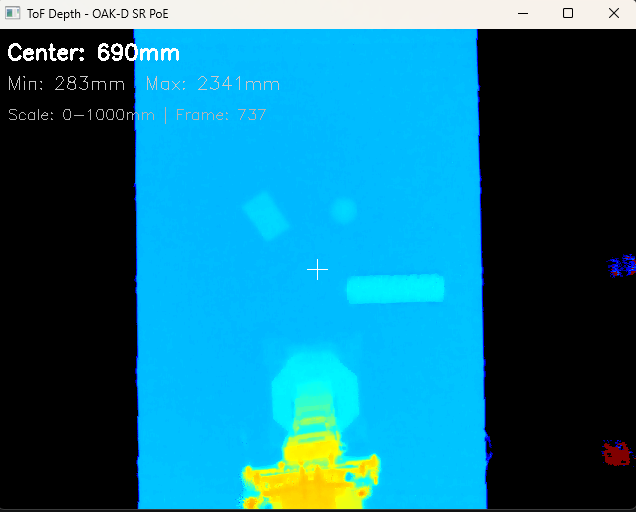
\includegraphics[width=\linewidth]{real_tof_depth.png}
\caption{Raw ToF depth (jet, $0$--$1000$\,mm).}
\end{subfigure}\hfill
\begin{subfigure}{0.40\textwidth}
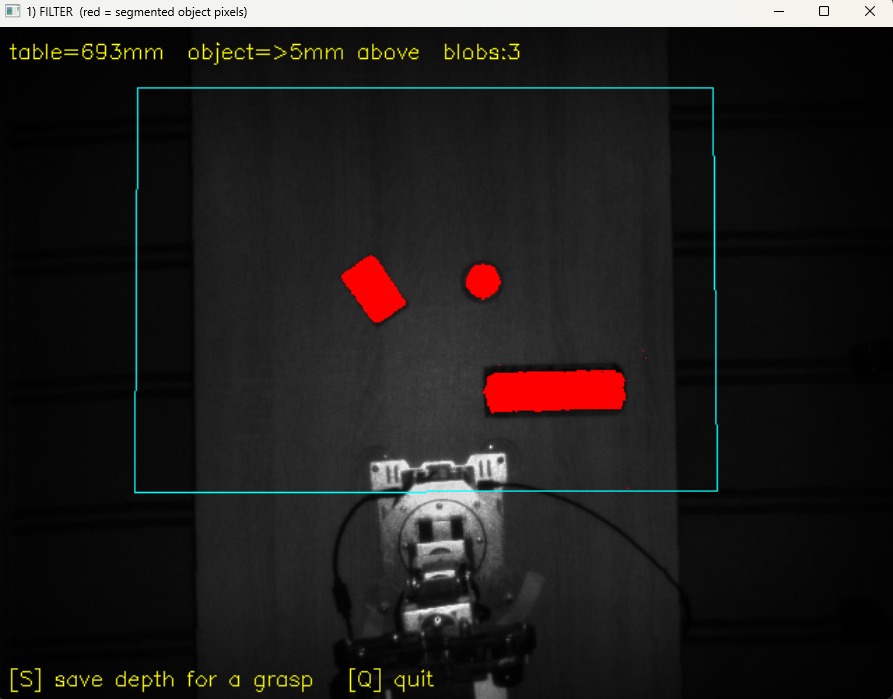
\includegraphics[width=\linewidth]{real_segmentation.png}
\caption{Depth segmentation: table plane at $693$\,mm; above-plane object blobs (red).}
\end{subfigure}
\caption{The physical system through the real overhead OAK-D SR PoE camera. \emph{(a)}~The
raw ToF depth stream (the planar table reads near-uniform; the arm enters from below).
\emph{(b)}~The same median-depth table removal used in simulation, run on the real frame:
the table plane is estimated at $693$\,mm and above-plane object pixels are segmented (red)
for median-centroid extraction.}
\label{fig:realrig}
\end{figure*}

\subsection{Objects}
The same four objects are used in every phase (Table~\ref{tab:objects}). They were chosen
to span a range of grasp difficulty, from a sharp-edged box that the jaws capture easily
to a slim can that nearly fills the gripper. Their grasp-relevant width sets the jaw
capture tolerance as $(55-w)/2$\,mm, where $55$\,mm is the measured real gripper opening.

\begin{table}[t]
\centering
\caption{The four test objects. The jaw capture tolerance is $(55-w)/2$\,mm, where $w$ is
the grasp width and $55$\,mm is the measured real gripper opening.}
\label{tab:objects}
\footnotesize
\resizebox{\columnwidth}{!}{%
\begin{tabular}{lcccl}
\toprule
Object & Width & Height & Jaw tol. & Character \\
       & (mm)  & (mm)   & (mm)     & \\
\midrule
coke\_can  & 52 & 47.3 & 1.5  & largest, fills the jaw \\
banana     & 35 & 26.1 & 10.0 & curved, elongated, 120\,g \\
golf\_ball & 43 & 29.6 & 6.0  & small, round, smooth \\
blue\_box  & 40 & 28.5 & 7.5  & sharp-edged, most robust \\
\bottomrule
\end{tabular}}
\end{table}

\subsection{Conditions}
The core conditions are \texttt{sim\_clean} (noise-free simulated depth),
\texttt{sim\_noisy\_oakd} (the model fitted to the measured OAK-D noise), and
\texttt{sim\_noisy\_nguyen} (the literature model). On top of these, the axial noise term
is swept with \texttt{axial\_scale}~$\in\{1,2,5,10,20\}$, where $\times1$ corresponds to
the measured noise and higher factors probe the estimator's robustness.

\subsection{Trials and metrics}
The pose experiment (Phase~3) was re-run on the current models with roughly 435 frames per
condition and 100\% detection. The simulated manipulation experiment (Phase~4A) is a
varied-placement sweep of 480 analytic trials: each object alone at 20 seeded positions and
orientations over the reachable annulus ($r$ from $0.12$ to $0.30$\,m, full yaw,
IK-validated, with the can lying down), crossed with the six noise conditions
($6\times4\times20$), giving $N=20$ per cell. The real perception experiment (Phase~4B)
uses five real scenes, yielding $n=4$ usable detections per object, because in most scenes
one object drifted into the unreliable ToF edge zone. The real manipulation experiment
(Phase~4C) uses all four objects, each at five placements with three repeats, for 60
trials.

The metrics are: translation RMSE and MAE in millimetres against ground truth (simulated
ground truth in simulation, ChArUco-referenced ground truth on the real system); the
analytic \texttt{grasp\_feasible} success rate as a percentage; and, for the real grasp,
lift-and-hold success with Wilson 95\% confidence intervals. Following the BOP convention,
alignment is taken on the visible top surface only \cite{hodan2018bop}; full 6D pose
metrics are not used because the estimator is translation-only. Detection-to-ground-truth
association uses greedy nearest-neighbour matching.

% =====================================================================

\section{Results}\label{sec:results}
\subsection{Real ToF noise characterisation (SQ1)}\label{sec:res-noise}
The planar protocol shows that axial precision is sub-millimetre and essentially flat with
range, with no Kinect-style growth (Table~\ref{tab:axial}, Figure~\ref{fig:sigma}).
Fitting the expected quadratic $\sigma_z(z)=a+bz^2$ gives $a=0.91$\,mm and a slightly
\emph{negative} curvature ($b\approx-0.49\,\mathrm{mm\,m^{-2}}$), so the Nguyen range model
\cite{nguyen2012modeling} does not apply here; the OAK-D's multi-frequency phase unwrapping
yields unusually quiet bulk depth (about $0.6$--$0.7$\,mm, against the $2$--$10$\,mm typical
of Kinect-class sensors). Bias stays within $\pm3$\,mm.

\begin{table}[t]
\centering
\caption{Planar axial precision versus distance (200 frames, $n\approx33{,}920$ px per
distance).}
\label{tab:axial}
\footnotesize
\begin{tabular}{lccccc}
\toprule
Distance (m)   & 0.40 & 0.50 & 0.60 & 0.70 & 0.80 \\
Axial $\sigma$ (mm) & 0.87 & 0.80 & 0.68 & 0.55 & 0.69 \\
\bottomrule
\end{tabular}
\end{table}

\begin{figure}[t]
\centering
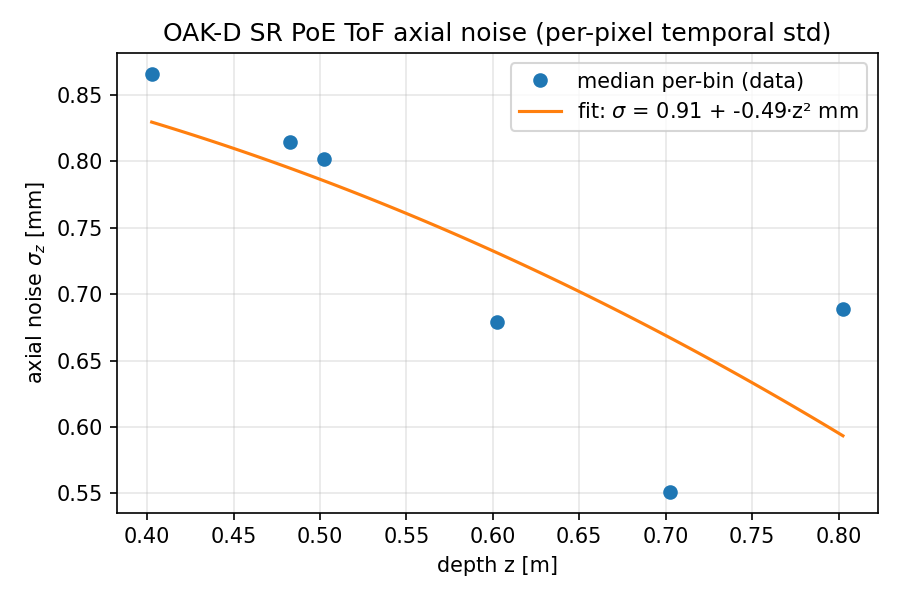
\includegraphics[width=\linewidth]{sigma_vs_z.png}
\caption{Axial depth precision $\sigma_z$ versus distance ($0.40$--$0.80$\,m). The profile
is sub-millimetre and flat (a slightly negative fitted curvature), so the range-growing
Nguyen model does not describe this multi-frequency ToF sensor.}
\label{fig:sigma}
\end{figure}

The object protocol locates the real, pose-relevant noise at object edges rather than on
their bodies (Table~\ref{tab:edge}, Figure~\ref{fig:overlays}). Body noise stays quiet on
all objects, but the six-pixel edge ring is dominated by flying pixels, with rates from
53\% to 99\%. This motivates both the median-centroid estimator and the inclusion of an
edge mixed-pixel term in the injector. Three caveats apply: the simple ``sharp edges are
clean, curved edges are noisy'' story is too strong, since the sharp box still shows
94.9\%; the can is low mainly because it is the largest object; and the rate is computed
over a fixed six-pixel ring, so it is partly size-sensitive and is reported qualitatively.

\begin{table}[t]
\centering
\caption{Per-object body noise and edge flying-pixel rate.}
\label{tab:edge}
\footnotesize
\begin{tabular}{lccc}
\toprule
Object & Body $\sigma$ (mm) & Dropout & Edge flying-pixel \\
\midrule
coke\_can  & 0.70 & 0\% & 53.1\% \\
banana     & 0.62 & 0\% & 98.7\% \\
golf\_ball & 0.65 & 0\% & 98.2\% \\
blue\_box  & 0.71 & 0\% & 94.9\% \\
\bottomrule
\end{tabular}
\end{table}

\begin{figure}[t]
\centering
\begin{subfigure}{0.49\linewidth}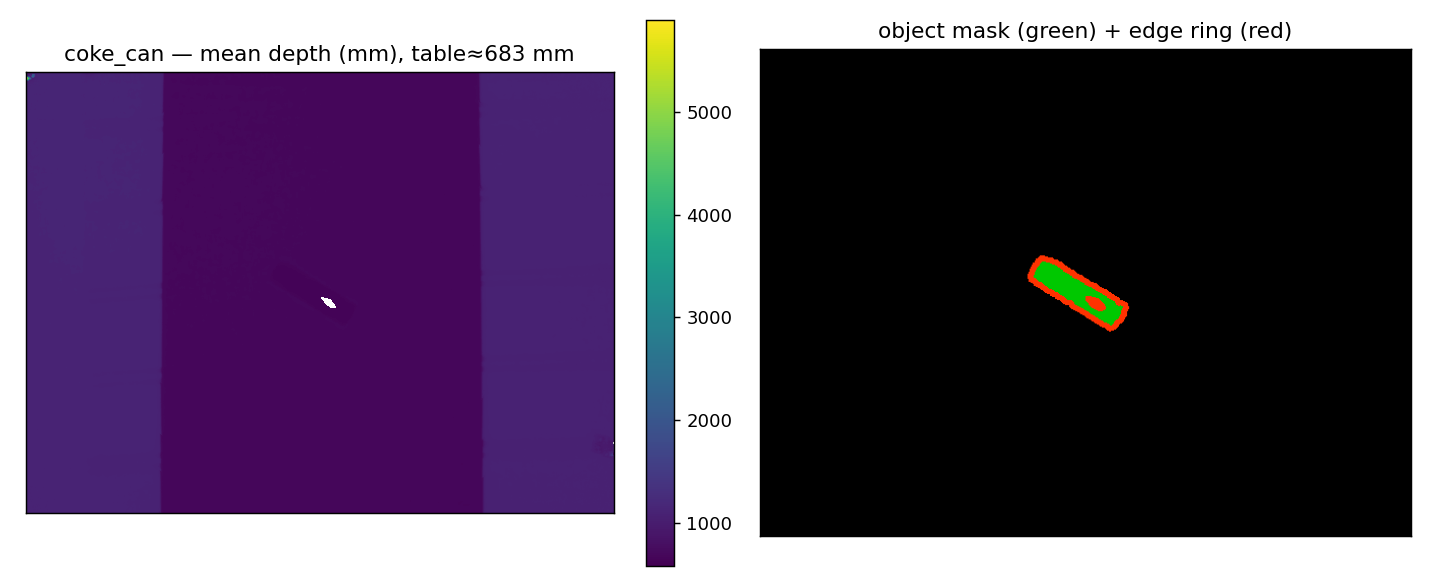
\includegraphics[width=\linewidth]{coke_can_overlay.png}\caption{coke\_can (53.1\%)}\end{subfigure}\hfill
\begin{subfigure}{0.49\linewidth}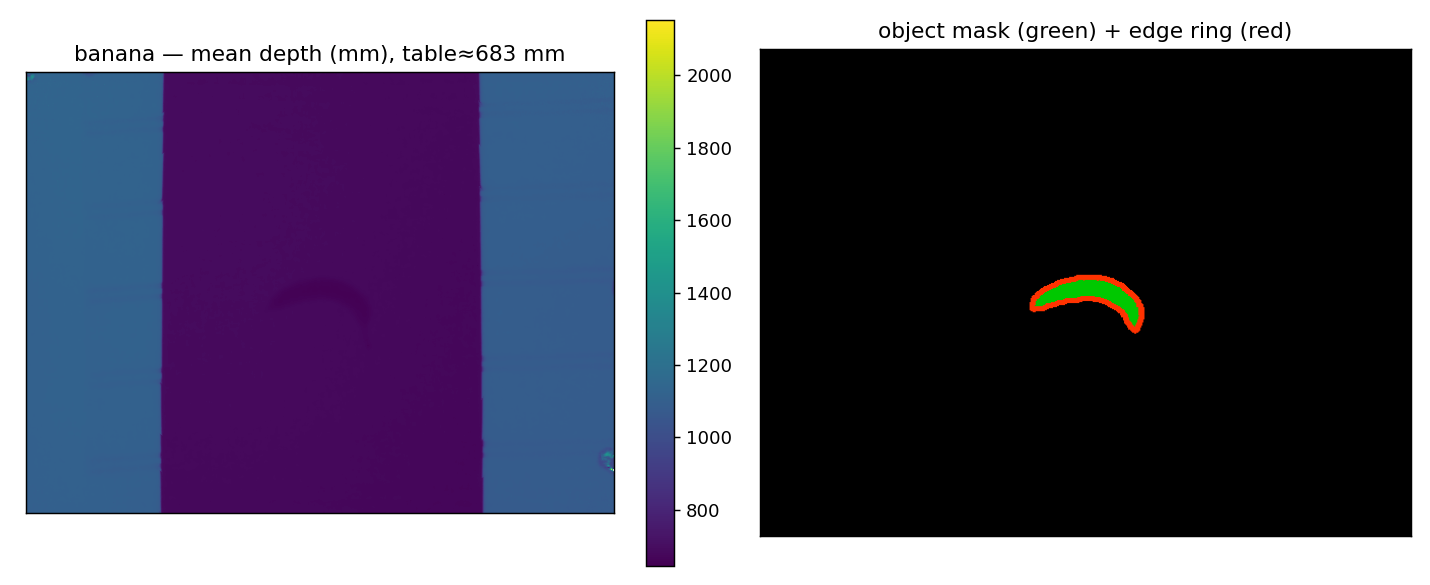
\includegraphics[width=\linewidth]{banana_overlay.png}\caption{banana (98.7\%)}\end{subfigure}
\\[2pt]
\begin{subfigure}{0.49\linewidth}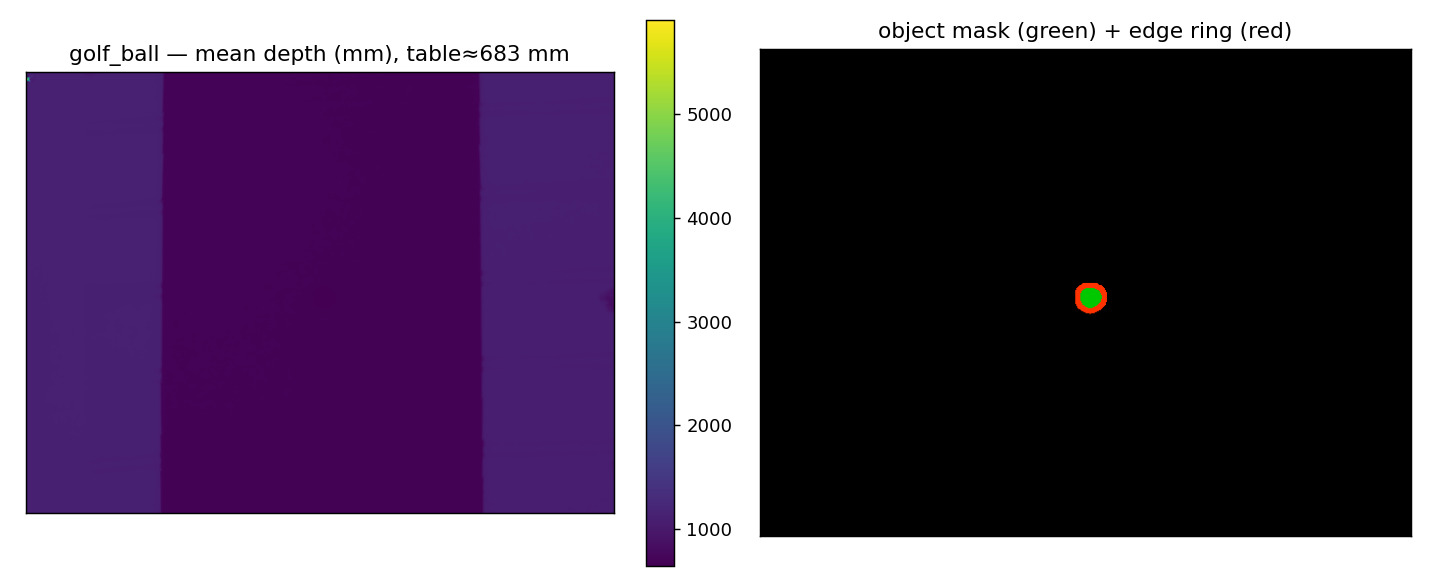
\includegraphics[width=\linewidth]{golf_ball_overlay.png}\caption{golf\_ball (98.2\%)}\end{subfigure}\hfill
\begin{subfigure}{0.49\linewidth}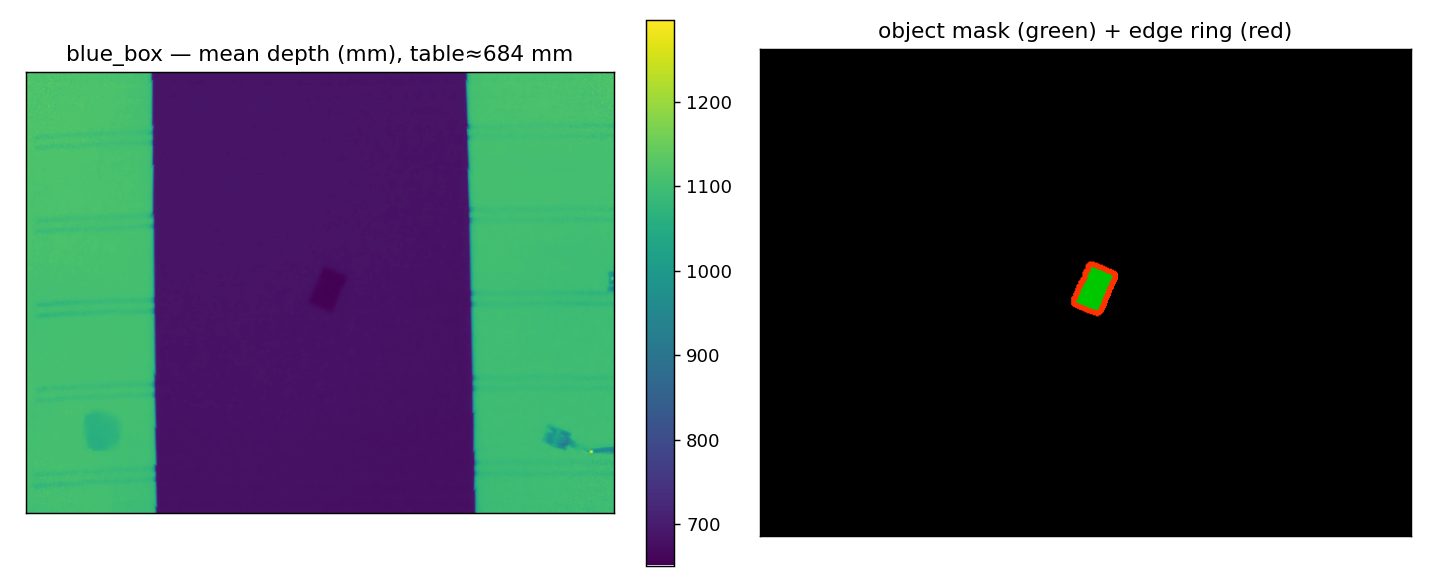
\includegraphics[width=\linewidth]{blue_box_overlay.png}\caption{blue\_box (94.9\%)}\end{subfigure}
\caption{Per-object edge overlays: the quiet body (green) versus the thin edge ring of
flying/mixed pixels (red). The pose-relevant noise lives almost entirely at the edges,
which the median centroid discards.}
\label{fig:overlays}
\end{figure}

\subsection{Noise injection and pose accuracy (SQ2)}\label{sec:res-inject}
At the measured noise level, injected noise has no measurable effect on pose accuracy. The
measured condition ($\times1$) is indistinguishable from clean and from the literature
model, and the planar (table-XY) RMSE stays flat at roughly $3.5$\,mm through $\times10$
(Table~\ref{tab:pose}, Figure~\ref{fig:posevsnoise}). The only visible movement below
$\times10$ is a small creep in the 3D RMSE, which is the axial (Z) component; the planar
difference between clean and $\times1$ is below $0.1$\,mm.

\subsection{Axial-scale ablation}\label{sec:res-ablation}
The same data are the ablation. Accuracy only degrades once the axial term is scaled to
about ten times the measured level (an axial $\sigma$ of roughly $9$\,mm), and all four
objects collapse together at $\times20$. This is the key verification that the null is real
rather than a broken pipeline: the injector does eventually break perception, but only an
order of magnitude above reality. That level is not merely hypothetical: an axial
$\sigma$ near $9$\,mm is representative of ToF operation in adverse conditions---strong
ambient infrared (e.g.\ direct sunlight), hot or industrial settings, airborne
particulates, and specular or low-reflectivity surfaces
\cite{foix2011lockin,sarbolandi2015kinect}---so the ablation also locates the regime in
which depth-noise fidelity would begin to matter (discussed in
Section~\ref{sec:disc-scope}).

\begin{table}[t]
\centering
\caption{Pose RMSE (mm) as planar\,/\,3D, by object and axial scale ($\times1$ is the
measured level). Values are flat from clean through $\times10$ and collapse at $\times20$.}
\label{tab:pose}
\footnotesize
\setlength{\tabcolsep}{4pt}
\resizebox{\columnwidth}{!}{%
\begin{tabular}{lcccc}
\toprule
Axial scale & coke\_can & banana & golf\_ball & blue\_box \\
\midrule
0 (clean)       & 3.31\,/\,4.85 & 8.71\,/\,10.67 & 4.77\,/\,7.89  & 3.06\,/\,3.06 \\
$\times1$       & 3.45\,/\,4.99 & 8.60\,/\,10.64 & 4.66\,/\,7.94  & 3.44\,/\,3.44 \\
$\times5$       & 3.53\,/\,6.03 & 8.68\,/\,11.12 & 4.53\,/\,8.55  & 3.63\,/\,3.71 \\
$\times10$      & 3.47\,/\,7.41 & 9.08\,/\,12.19 & 4.39\,/\,10.48 & 3.44\,/\,4.03 \\
$\times20$      & 9.55\,/\,18.43 & 22.43\,/\,24.53 & 8.58\,/\,19.08 & 8.68\,/\,10.21 \\
\bottomrule
\end{tabular}}
\end{table}

\begin{figure}[t]
\centering
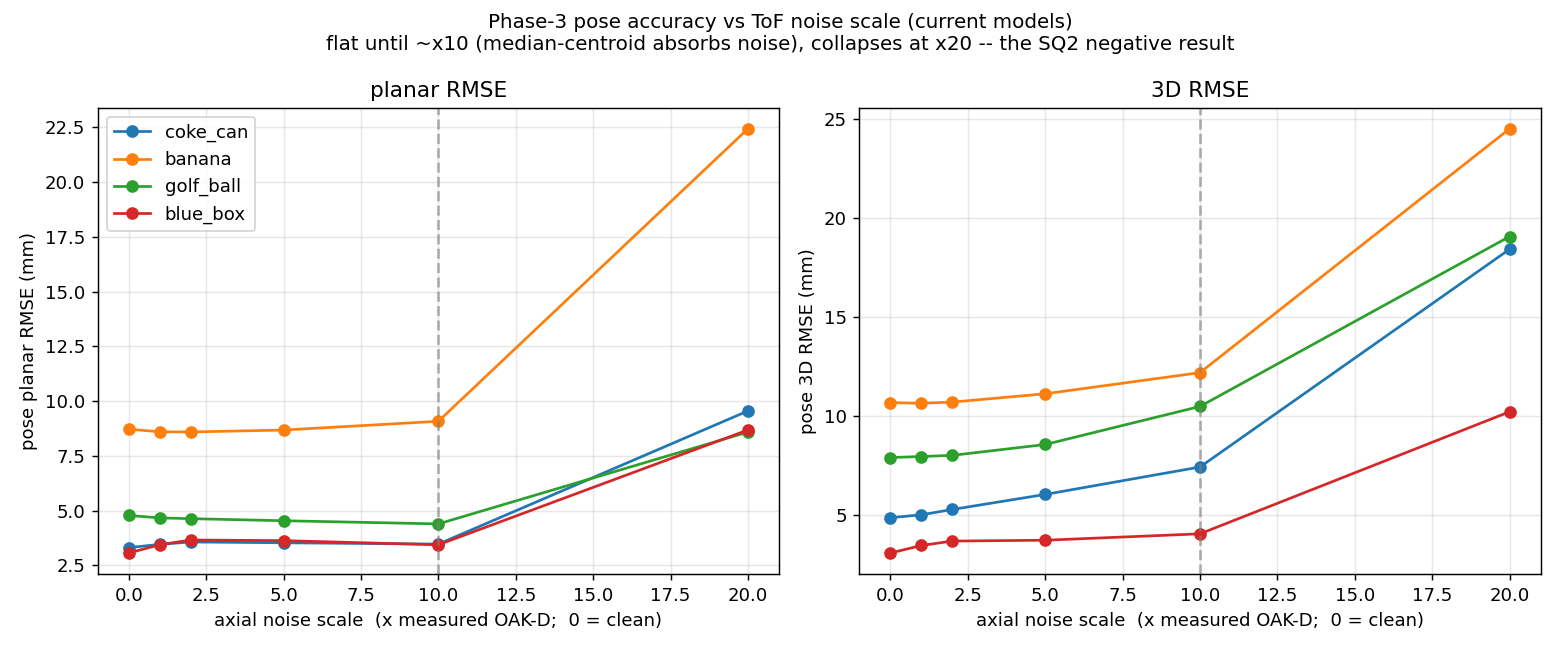
\includegraphics[width=\linewidth]{phase3_pose_vs_noise.png}
\caption{Pose RMSE versus axial noise scale for the four objects: flat from clean through
$\times10$, then a sharp collapse at $\times20$. Realistic noise ($\times1$) sits an order
of magnitude below the threshold at which the estimator degrades.}
\label{fig:posevsnoise}
\end{figure}

\subsection{Simulated manipulation (SQ3, simulation)}\label{sec:res-simmanip}
The simulated grasp results echo the pose threshold (Table~\ref{tab:grasp},
Figure~\ref{fig:rate}). All four objects are detected in every trial, so accuracy rather
than detection is the bottleneck. The three graspable objects are flat from clean through
$\times10$ and collapse only at $\times20$. Per-object behaviour is governed by the clean
error against the jaw tolerance: the blue box (${\sim}3.5$\,mm error against a $7.5$\,mm
tolerance) is at 100\%; the golf ball (${\sim}5.2$ against $6.0$) and banana
(${\sim}9.3$ against $10$) sit on their tolerance boundaries at 65\%; and the can
(${\sim}4.9$ against $1.5$) is floored at 0\%, a size limit ($52$\,mm body in a $55$\,mm
jaw) rather than a noise effect.

\begin{table}[t]
\centering
\caption{Analytic \texttt{grasp\_feasible} success rate (\%), $N=20$ per cell. Jaw
tolerance per object in parentheses.}
\label{tab:grasp}
\footnotesize
\setlength{\tabcolsep}{4pt}
\resizebox{\columnwidth}{!}{%
\begin{tabular}{lccccc}
\toprule
Condition & coke & banana & golf & blue\_box & Overall \\
          & (1.5) & (10) & (6) & (7.5) & \\
\midrule
clean         & 0  & 65 & 65 & 100 & 57.50 \\
$\times1$     & 5  & 65 & 65 & 100 & 58.75 \\
$\times10$    & 0  & 65 & 75 & 100 & 60.00 \\
$\times20$    & 5  & 30 & 20 & 50  & 26.25 \\
\bottomrule
\end{tabular}}
\end{table}

\begin{figure}[t]
\centering
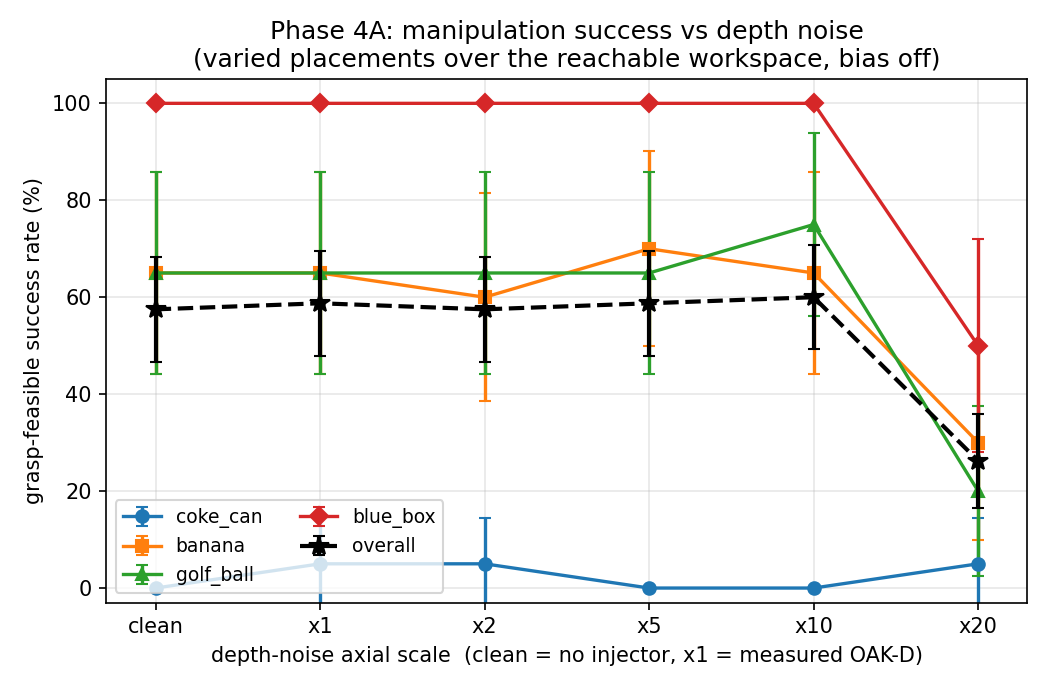
\includegraphics[width=\linewidth]{phase4a_rate_vs_axial_scale.png}
\caption{Analytic grasp-feasible success versus axial noise scale, per object. The three
graspable objects are flat clean$\rightarrow\times10$ and collapse at $\times20$; the can
is floored by a size limit independent of noise.}
\label{fig:rate}
\end{figure}

\subsection{Real pose gap and real manipulation (SQ3, real)}\label{sec:res-real}
The negative result carries onto the real system. The measured real-versus-sim planar pose
gap is small for every object, between $-1.4$ and $+3.6$\,mm (Table~\ref{tab:gap},
Figure~\ref{fig:gap}), and \texttt{sim\_clean} remains indistinguishable from
\texttt{sim\_noisy\_oakd} on real data. The simulated reference here is the
varied-placement sweep of Section~\ref{sec:res-simmanip}, whose wider pose spread raises
planar RMSE relative to the central scenes of Table~\ref{tab:pose}; this is why the
\texttt{sim\_clean} values differ between the two tables. The one positive outlier is the
blue box ($+3.6$\,mm), which becomes relevant for grasping.

\begin{table}[t]
\centering
\caption{Real-versus-sim planar pose RMSE (mm). The gap is computed as
real\,$-$\,\texttt{sim\_clean}.}
\label{tab:gap}
\footnotesize
\setlength{\tabcolsep}{4pt}
\resizebox{\columnwidth}{!}{%
\begin{tabular}{lcccc}
\toprule
Condition & coke\_can & banana & golf\_ball & blue\_box \\
\midrule
sim\_clean ($n{=}20$)      & 10.44 & 13.27 & 6.15 & 3.78 \\
sim\_noisy\_oakd ($n{=}20$) & 10.35 & 13.24 & 6.02 & 3.54 \\
real ($n{=}4$)             & 9.38 & 12.13 & 4.75 & 7.42 \\
\midrule
Gap (real $-$ sim\_clean)  & $-1.1$ & $-1.1$ & $-1.4$ & $+3.6$ \\
\bottomrule
\end{tabular}}
\end{table}

\begin{figure}[t]
\centering
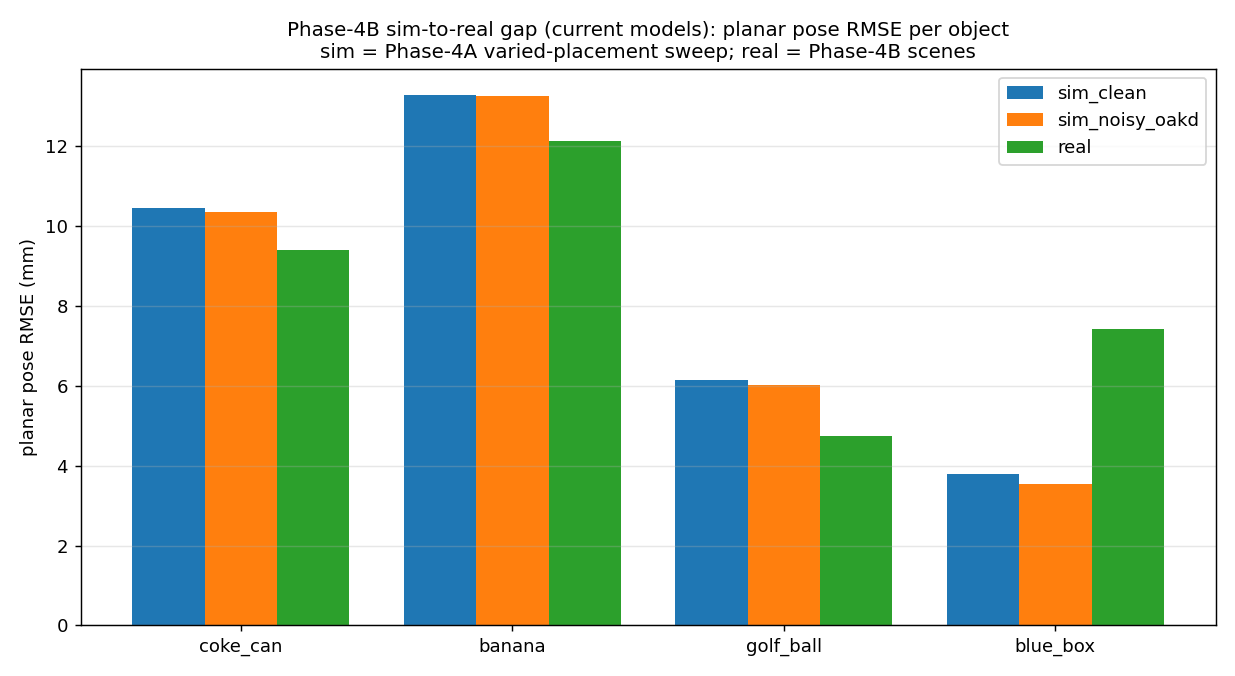
\includegraphics[width=\linewidth]{phase4b_sim_to_real_gap.png}
\caption{Real versus simulated planar pose RMSE per object (clean sim, noisy sim, real).
The real bars land close to the simulated ones, and clean and noisy simulation remain
indistinguishable: the negative result carries end-to-end on real data.}
\label{fig:gap}
\end{figure}

For real manipulation, all four objects were run under closed-loop control at five
near-zone placements with three repeats each, for 60 trials (Table~\ref{tab:phase4c},
Figure~\ref{fig:realpred}). The blue box reached 11/15 (73\%), the banana and coke can both
10/15 (67\%), and the golf ball 3/15 (20\%), for an overall $34/60=57\%$ lift-and-hold. The
most informative feature is that these rates follow neither the Phase-4A analytic
feasibility ceiling nor the Phase-4B pose-error-versus-tolerance predictor; they diverge
from both, and in both directions. Once the visual loop has driven the in-frame aiming
error to the camera floor (about $1$--$3$\,mm for every object in the near zone), the
residual variance is set by grip mechanics---object shape against the parallel-jaw closing
force and compliance---rather than by perception or aim.

The coke can is the clearest case. Its analytic feasibility is 0\% and its $1.5$\,mm rigid
centring tolerance predicts ``${\sim}0\%$'', yet it grasped 67\% of the time, so the real
arm out-performs the simulator: the loop centres the gripper to about $1$\,mm, and the firm
commanded close (well past the $52$\,mm body) stalls against the slightly compliant can with
enough force to secure it, an effect the rigid feasibility metric cannot represent. The
golf ball is the opposite. Its predictor was the most favourable of the four
($4.8<6.0$\,mm, ``likely''), yet it reached only 20\%, because a smooth sphere makes point
contact and rolls out of flat parallel jaws even when the aim converges below $2$\,mm; the
closed loop fixes the aim that was golf's wall but cannot supply a form-closure that flat
jaws do not afford a sphere. The banana (67\%) likewise exceeds its planar-RMSE prediction,
the elongated body being forgiving along its length. The blue box (73\%) is the only object
the predictor ``called''; within the validated near-zone ($r\le0.20$\,m, placements p1, p3,
p5) it grasped $9/9=100\%$, and every failure occurred at the far edge ($r\ge0.22$\,m), where
the high-mounted gripper marker loses tracking gain (Table~\ref{tab:bluebox}).

\begin{table*}[t]
\centering
\caption{Phase-4C real lift-and-hold success on the physical arm (60 trials), beside the
Phase-4A analytic feasibility ceiling and the Phase-4B pose-error-versus-tolerance
predictor. Intervals are Wilson 95\% score intervals.}
\label{tab:phase4c}
\footnotesize
\begin{tabular}{lccccccc}
\toprule
Object & $N$ & lift $k$ & rate (\%) & 95\% CI & sim-feas.\ (\%) & pose err (mm) & jaw tol (mm) \\
\midrule
blue\_box  & 15 & 11 & \textbf{73} & $[48,89]$ & 100 & 7.4  & 7.5 \\
banana     & 15 & 10 & \textbf{67} & $[42,85]$ & 65  & 12.1 & 10.0 \\
coke\_can  & 15 & 10 & \textbf{67} & $[42,85]$ & 0   & 9.4  & 1.5 \\
golf\_ball & 15 & 3  & \textbf{20} & $[7,45]$  & 65  & 4.8  & 6.0 \\
\midrule
\textbf{overall} & 60 & 34 & \textbf{57} & $[44,68]$ & --- & --- & --- \\
\bottomrule
\end{tabular}
\end{table*}

\begin{figure*}[t]
\centering
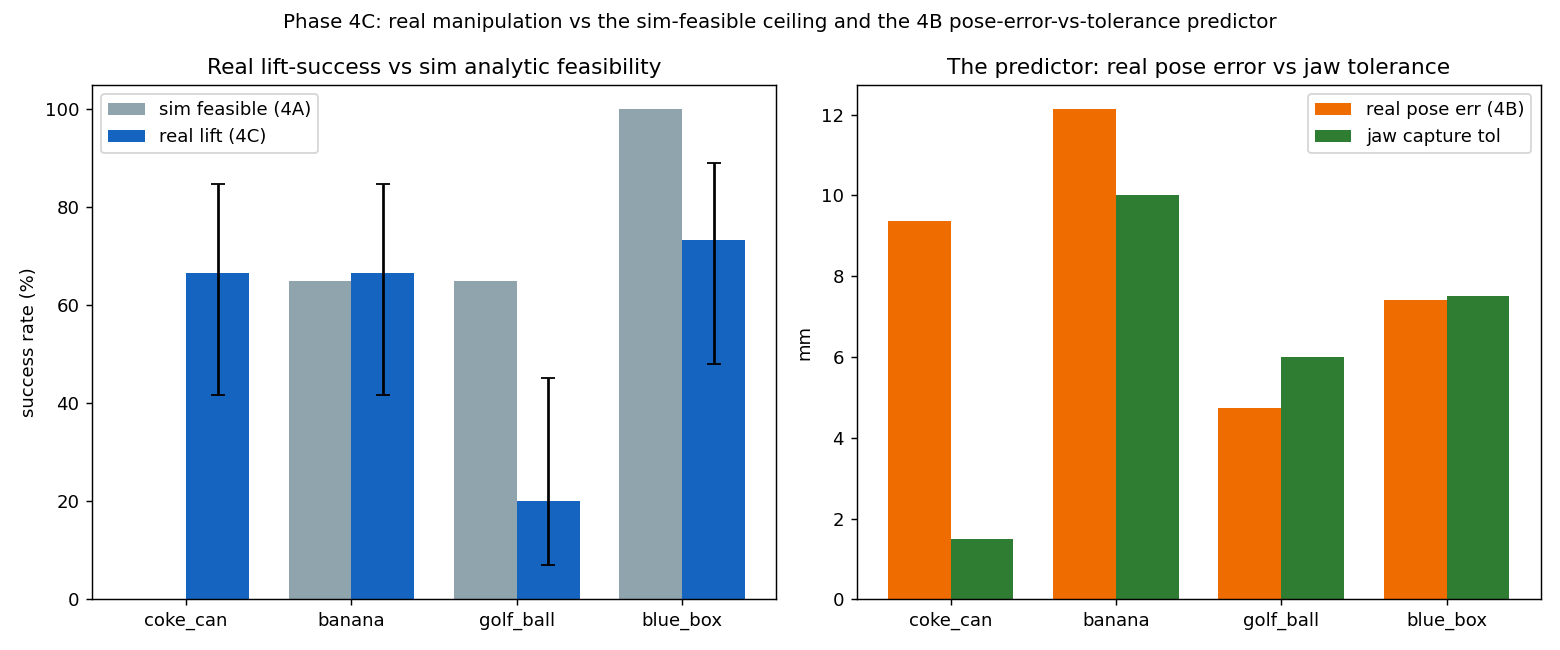
\includegraphics[width=0.9\textwidth]{phase4c_real_vs_pred.png}
\caption{Phase-4C real manipulation. \emph{Left:} real lift-success (with Wilson 95\%
intervals) against the Phase-4A analytic feasibility ceiling; the coke can has no
feasibility bar (0\%) yet grasps 67\%, while the golf ball has a 65\% ceiling yet only 20\%
real success. \emph{Right:} the Phase-4B planar pose error against each object's jaw
tolerance, which likewise fails to order the real rates---success is set by grip mechanics,
not aim.}
\label{fig:realpred}
\end{figure*}

\begin{table}[t]
\centering
\caption{Phase-4C closed-loop blue-box trials (5 placements $\times$ 3 repeats). The servo
column is the table-frame alignment error before$\rightarrow$after the visual nudge (mm).}
\label{tab:bluebox}
\footnotesize
\setlength{\tabcolsep}{4pt}
\resizebox{\columnwidth}{!}{%
\begin{tabular}{lcll}
\toprule
Placement & Reach $r$ & Servo error (mm) & Outcome \\
\midrule
p1 (0.35,0.16) & 0.20 & 20$\to$2, 23$\to$2, 23$\to$2 & OK, OK, OK \\
p2 (0.31,0.22) & 0.22 & 26$\to$7, 31$\to$8, 24$\to$2 & OK, fail, OK \\
p3 (0.37,0.29) & 0.16 & 16$\to$2, 17$\to$2, 16$\to$3 & OK, OK, OK \\
p4 (0.30,0.34) & 0.23 & 44$\to$17, 40$\to$11, 40$\to$11 & fail, fail, fail \\
p5 (0.37,0.37) & 0.19 & 34$\to$2, 31$\to$2, 33$\to$3 & OK, OK, OK \\
\bottomrule
\end{tabular}}
\end{table}

% =====================================================================

\section{Discussion}\label{sec:discussion}
\subsection{A valid negative result, not a broken pipeline}
The central outcome of this thesis is negative: at the noise level actually measured on the
OAK-D SR PoE, injecting a fitted ToF noise model into simulation does not change pose
accuracy (Section~\ref{sec:res-inject}) and does not change simulated grasp feasibility
(Section~\ref{sec:res-simmanip}). This refutes the proposal hypothesis. The result is sound
rather than an artefact of an insensitive pipeline, because the same injector does degrade
perception once the axial term is scaled up: pose error grows only past roughly $\times10$
measured noise ($\sigma\approx9$\,mm) and manipulation collapses only at $\times20$
(Section~\ref{sec:res-ablation}). Realistic noise simply sits an order of magnitude below
the level at which it begins to matter.

\subsection{The scope of the null: benign versus harsh environments}
\label{sec:disc-scope}
The negative result is not a claim that ToF noise never matters; it is a claim about a
specific---and very common---operating regime. All of the noise measured in this work was
recorded indoors under controlled, diffuse lighting, where the OAK-D's multi-frequency
phase unwrapping keeps axial precision sub-millimetre (Section~\ref{sec:res-noise}). The
ablation (Section~\ref{sec:res-ablation}) is the other half of the story: the estimator
\emph{does} break once the axial term is scaled to roughly $\times10$ ($\sigma\approx9$\,mm),
and grasping collapses by $\times20$ ($\sigma\approx18$\,mm). Crucially, these are not
arbitrary stress levels---they are the levels that ToF cameras genuinely reach \emph{outside}
the benign indoor regime. Under strong ambient infrared such as direct sunlight, in hot or
industrial settings, in airborne particulates (dust, fog, smoke), on specular or dark
low-reflectivity surfaces, and at extended range, ToF axial error is well documented to grow
by an order of magnitude or more, driven by a reduced signal-to-background ratio, increased
shot and thermal noise, and multipath \cite{foix2011lockin,sarbolandi2015kinect}. The
practical reading of the negative result is therefore \emph{conditional on the environment}.
For an indoor or office tabletop system---the setting this thesis targets---modelling
realistic depth noise is not worth the effort, because the operating point sits an order of
magnitude below the level at which noise reaches the median-centroid estimate. For a system
meant to run outdoors, in a hot or hazardous industrial environment, or at long range, the
same analysis predicts the opposite: the operating point moves into the $\times10$--$\times20$
band where injected noise demonstrably degrades both pose accuracy
(Table~\ref{tab:pose}) and grasp success (Table~\ref{tab:grasp}), and there a faithful
ToF-noise model---together with a perception front-end designed to tolerate it---would pay
off. The ablation should thus be read not as a curiosity an order of magnitude from reality,
but as a map of the boundary between these two regimes, and it is the regime, not the noise
model alone, that decides whether depth-noise fidelity is worth modelling.

\subsection{Why the estimator absorbs realistic noise}
The pose-relevant noise on the real sensor does not live in the body of each object but in
a thin ring of edge mixed-pixels, whose flying-pixel rate reaches 53 to 99\% across the
four objects while the bulk axial precision stays below $1$\,mm
(Section~\ref{sec:res-noise}). A per-axis median centroid (Section~\ref{sec:methods-perc})
has a 50\% breakdown point \cite{huber1981robust}, so it rejects this edge population as
long as the outliers stay a minority of the blob. The injected axial Gaussian, by contrast,
perturbs the quiet body pixels that the median already estimates well, so it has almost no
leverage on the centroid. This also reframes the literature models: rather than adopting
Nguyen's quadratic range term blindly, the Phase~2 data test it and find it inapplicable to
this multi-frequency sensor \cite{nguyen2012modeling}.

\subsection{Where the gap actually lives}
If depth-noise fidelity does not govern the gap, what does? The real-versus-sim planar pose
comparison (Section~\ref{sec:res-real}) puts the end-to-end gap at $-1.4$ to $+3.6$\,mm
across all four objects, with clean and noisy simulation still indistinguishable on real
data. The residual is consistent with calibration and lighting rather than sensor
stochasticity: the extrinsic is a single direct \texttt{solvePnP} solution, factory
intrinsics are used without a dedicated calibration run, and segmentation quality varies
with illumination at the object boundary. This echoes the broader lesson of domain
randomisation work, that the factors which dominate transfer are often not the ones a given
pipeline randomises \cite{tobin2017domain}, and it locates the reality gap
\cite{jakobi1995noise} for this system in geometry and photometry rather than in the
depth-noise statistics.

\subsection{Manipulation: the real bottleneck is kinematic, and grip mechanics decide}
The manipulation results separate two error sources. In simulation, grasp feasibility is
governed purely by perceived-centre error against jaw tolerance, so the three objects with
adequate tolerance are flat from clean through $\times10$ and only the size-limited coke can
is floored. On the real arm, the dominant error is not perception but the kinematic model:
the xArm~1S over-reaches its URDF by roughly 28\%, and a global similarity-scale workaround
leaves about $14$\,mm of residual position error, more than the blue box's $\pm7.5$\,mm
capture tolerance, which confined open-loop grasping to a narrow patch. The closed-loop
visual nudge (Section~\ref{sec:methods-servo}) removes this by construction: because the
error is a difference between two points seen through the same overhead camera in the same
frame, the wrong forward kinematics and the scale factor cancel as common-mode bias, and
grasp accuracy becomes camera-bound rather than model-bound. With aiming corrected, the
per-object grasp rates (Table~\ref{tab:phase4c}) are ordered by neither the simulated
feasibility ceiling nor the measured pose error, but by the interaction of object shape with
the parallel-jaw closing force: the coke can rises from a predicted 0\% to 67\% (a firm close
on a slightly compliant, near-jaw-width can), while the golf ball falls from a favourable
65\% prediction to 20\% (a smooth sphere that rolls out of flat jaws). This is consistent
with the grasping literature's distinction between geometric reachability and grasp
stability \cite{bohg2014grasp}.

\subsection{Simulation realism and the analytic metric}
A deliberate scoping choice shapes how the simulated manipulation numbers should be read.
Gazebo Classic \cite{koenig2004gazebo} cannot reliably resolve contact grasps on small or
curved objects in this setup; finger collisions pass through and object pose is unchanged
across a jaw close. The simulated success metric is therefore analytic grasp feasibility,
not scored physical contact, and it was renamed accordingly to avoid overclaiming. This
keeps every simulated error attributable to perception, but it means the simulated rates are
an upper bound on what a physical grasp would achieve. The contact-attach plugin
\cite{link_attacher} is used only for visualisation.

\subsection{Limitations}
Several limitations bound the strength of these claims. The real perception comparison is
$n=4$ per object: in four of five scenes one object drifted into the ToF edge zone and
failed to segment, because the reliable ToF area is smaller than the RGB marker field of
view. The real manipulation evaluation covers all four objects (60 trials) but is restricted
to the near workspace ($r\le0.20$\,m); beyond that radius the loop gain falls because the
marker is mounted high and behind the jaws, a known mounting issue rather than a limit of the
method. The Phase-4A confidence intervals are Wald and collapse to zero width at 0\% and
100\%, so the Wilson intervals used in Phase~4C are the more honest choice. The noise model
omits spatial correlation and multipath, and the lateral jitter term uses the literature
value of $0.8$\,px \cite{nguyen2012modeling} rather than a separately measured one. Finally,
Gazebo Classic reached end of life in January~2025, so while the simulation results are
stable they rest on an unsupported platform. None of these affect the central negative
result, which is established independently in Phases~2 and~3 and corroborated on real data in
Phase~4B.

% =====================================================================

\section{Conclusion and Future Work}\label{sec:conclusion}

\paragraph{Summary of main contributions.}
This thesis asked how modelling realistic ToF sensor noise affects the sim-to-real gap in
RGB-D tabletop pose estimation and manipulation, and answered it through five connected
phases. It contributes (i) a measured ToF characterisation showing that the OAK-D's bulk
depth is sub-millimetre and flat with range while the pose-relevant noise is concentrated in
edge flying-pixels; (ii) a verified four-term injection module; (iii) the central negative
result---for a depth-segmented median-centroid estimator, injecting measured ToF noise has no
measurable effect on pose RMSE (under $0.1$\,mm versus clean) and none on grasp feasibility,
with degradation appearing only near $\times10$ ($\sigma\approx9$\,mm) for pose and $\times20$
for manipulation; (iv) end-to-end real validation, a $-1.4$ to $+3.6$\,mm real-versus-sim
planar gap and a $34/60$ ($57\%$) closed-loop real grasp rate (100\% for the aiming-limited
blue box inside the near-zone); and (v) a reproducible Gazebo/ROS~2 setup. The synthesis is
that, for this class of estimator, the sim-to-real gap is not governed by depth-noise-model
fidelity; it lives in calibration, lighting, and segmentation, and on the real arm the single
largest source is an open-loop kinematic-model error that one visual-feedback correction
removes within its working range. With aim corrected, the per-object real rates are set by
grip mechanics rather than perception. Crucially, this null is \emph{conditional on the
operating environment}: the same ablation shows that once depth noise reaches the level
typical of harsh, hot, or outdoor ToF operation---about $\times10$ the indoor measurement
($\sigma\approx9$\,mm)---it does degrade both pose and grasp success, so for a system
intended to leave the controlled indoor regime, faithful depth-noise modelling becomes
worthwhile (Section~\ref{sec:disc-scope}).

\paragraph{Future work.}
The clearest hardware lever is a gripper better matched to round and near-jaw-width objects:
compliant fingertip pads or a small cradle would address the golf ball's roll-out and further
stabilise the coke can's forceful grip. Mounting the gripper marker low and directly over the
jaw gap, so that it tracks the fingertips one-to-one, should extend reliable convergence to
the full reach. The arm-base calibration could be re-solved with more touch points or replaced
by a learned dense-correction field in the style of low-cost reproducible-arm work
\cite{yang2019replab}. On the perception side, the noise model could be extended to capture
spatial correlation and multipath, and the median-centroid baseline could be compared against
a learned pose or grasp model such as MVGrasp \cite{kasaei2021mvgrasp} to test whether a
data-driven estimator is more or less sensitive to the same edge noise. Characterising the
OAK-D in outdoor, dusty, or high-temperature conditions would directly test the predicted
crossover into the noise-limited regime (Section~\ref{sec:disc-scope}), where these
extensions would matter most. Finally, repeating the
simulated manipulation on a contact-capable physics backend would let the analytic feasibility
metric be validated against scored physical grasps.

% =====================================================================


% --- references (APA / apacite) ---
\bibliographystyle{apacite}
\bibliography{references}

% --- appendices (one file each) ---
\appendix
\onecolumn
\section{Assets and Attribution}\label{app:assets}
This appendix records the third-party assets and software used in the project.

\paragraph{3D models.} The xArm~1S robot description (URDF and meshes) is adapted from a
community-maintained model published on GrabCAD by Yair Casas \cite{grabcad_xarm}. The
coke-can mesh is ``Soda Can 250ml'' by sebastian204 \cite{sketchfab_cokecan} and the banana
mesh is ``Banana'' by Lassi Kaukonen \cite{sketchfab_banana}, both on Sketchfab under
CC-BY-4.0. The golf ball and blue box are simulation primitives (a sphere and a box) with no
external mesh, and the coke can is modelled as a slim primitive cylinder.

\smallskip\noindent\emph{Required CC-BY-4.0 attribution.} This work is based on ``Soda Can
250ml'' (\url{https://sketchfab.com/3d-models/soda-can-250ml-557bd388b7b340a88053016f39c3d514})
by sebastian204, and ``Banana''
(\url{https://sketchfab.com/3d-models/banana-dda3a1f707a94c52bed79578e120937c}) by Lassi
Kaukonen, both licensed under CC-BY-4.0 (\url{http://creativecommons.org/licenses/by/4.0/}).

\paragraph{Software.} The simulation uses Gazebo Classic~11 \cite{koenig2004gazebo} with
ROS~2 Humble \cite{macenski2022ros2} and a vendored \texttt{gazebo\_ros2\_control}
\cite{gazebo_ros2_control}. The custom contact-triggered attach plugin follows the
IFRA-Cranfield link-attacher pattern \cite{link_attacher} and is used for visualisation only.
Perception uses OpenCV \cite{bradski2000opencv} and the tf2 transform library
\cite{foote2013tf}; fiducials use ArUco and ChArUco
\cite{garridojurado2014aruco,romeroramirez2018charuco}. The real camera is driven through
DepthAI \cite{depthai_docs} on the Luxonis OAK-D SR PoE \cite{luxonis_oakd}.

\section{Declaration of Originality and Use of AI Tools}\label{app:declaration}
I declare that this thesis and the work it reports are my own and were carried out under the
supervision of Dr.\ H.\ Kasaei. All sources and third-party assets are acknowledged in the
references and in Appendix~\ref{app:assets}.

I used AI-based tools (large language model assistants) during the project, for example to
help draft and revise text, to help structure and debug code, and to organise notes. All
experimental design, data collection, analysis, and final results are my own, and I take full
responsibility for the content of this thesis. The specific tools and the manner of their use
are disclosed in line with the University of Groningen policy on the use of AI in education.

\section{Reproducibility and Repository}\label{app:repro}
The full ROS~2 workspace, perception and noise-injection code, evaluators, and the result
files that back every table and figure are available in the project repository. The headline
numbers are reproducible from the comma-separated result files (Phase-3 pose table, Phase-4A
success table, Phase-4B gap table, and the Phase-4C trial log) using the summary scripts in
the \texttt{evaluation} package. The software stack is Gazebo Classic~11, ROS~2 Humble,
DepthAI~v3.5, and Python~3.


\end{document}
